% Re-defined by Z.C.TIAN (https://github.com/doem97)
% This version comply with the Official EEE Dissertation Guidline in [EEE dissertation] (http://www.eee.ntu.edu.sg/programmes/CurrentStudents/Graduate_Coursework/mscProg/disHome/Pages/home.aspx)
% More information about dissertation can be found in [NTU thesis](http://research.ntu.edu.sg/rieo/RI/Pages/Theses--Dissertations.aspx)
% Based on W.M.ZHAO version, original link in overleaf:
% (https://www.overleaf.com/latex/templates/ntu-master-dissertation/ngnhrrwryccv)

\documentclass[12pt]{report}

%% Useful packages
\usepackage[a4paper,top=3cm,bottom=3cm,left=3.5cm,right=3cm,marginparwidth=1.75cm,headheight=22pt]{geometry}
\usepackage{amsmath}
\usepackage{cite}
\usepackage{courier}
\usepackage{minted} % For highlighted source code
\usepackage[titletoc]{appendix}
\usepackage[export]{adjustbox}
\usepackage[nottoc,notlot,notlof]{tocbibind}
\usepackage[labelfont=bf, textfont=bf]{caption}
\usepackage{graphicx}
\usepackage{booktabs}
\usepackage[bottom]{footmisc}
\usepackage{hyperref}
\usepackage{float}
\usepackage{setspace}
\usepackage{subfigure}
\usepackage{setspace}
\usepackage{lipsum}
\usepackage{fancyhdr} % Fancy header
\usepackage{url}
\usepackage{tabularx}
\usepackage[utf8]{inputenc}
\usepackage{mathptmx} %Times Font

%==== Header and Footer configure ====
% Define the plain pagestyle used by most chapters
\fancypagestyle{plain}{
\fancyhf{} % Clear header footer
\fancyhead[R]{\bf \small \textsl{\nouppercase{\leftmark}} \vspace{0.1in}}
\fancyfoot[R]{\thepage}
% Set the right side of the footer to be the page number
\renewcommand{\headrulewidth}{2pt}
}

%==== Overall Config ====
\setlength{\parindent}{0in} % Set paragraph indent as 0
% \setlength{\fboxsep}{-0.3in}%
\setlength{\fboxrule}{0.5pt} % Set the bounding box around the image as 0.5pt
\pagestyle{plain}
% \renewcommand{\chaptermark}[1]{\markboth{#1}{}}% Comment this line to use header "Chapter 1. Literature View"; otherwise header is "Literature View"



\begin{document}
\fontdimen2\font=0.5em% inter word space
%==== FRONT PART====
\begin{titlepage}

\begin{figure}[h!]
\centering

\includegraphics[width=1\textwidth]{Title/NTU-LOGO-bw.pdf}
\caption*{}
\label{fig:entropy} 
\end{figure}

\vspace{1.5in}

\centering
\Huge{\textbf{Your Title of the Dissertation\\Also Second Line}}\\[2.5in]

\LARGE{\textbf{YOUR NAME}}\\[0.5in]

\normalsize{\textbf{SCHOOL OF ELECTRICAL AND ELECTRONIC ENGINEERING}}\\[0.2in]

% \textbf{A DISSERTATION SUBMITTED IN PARTIAL FULFILMENT OF\\
% THE REQUIREMENTS FOR THE DEGREE OF\\
% MASTER OF SCIENCE IN DIGITAL MEDIA TECHNOLOGY}\\[0.25in]

\large{\textbf{2021}}
\end{titlepage}
\newpage % Coverpage
\begin{titlepage}
\begin{center}
\vspace*{2in}
\Huge{\textbf{Your Title of the Dissertation\\Also Second Line}}\\[2.5in]

\LARGE{\textbf{\MakeUppercase{YOUR NAME}}}\\[1in]

\normalsize{\textbf{\MakeUppercase{SCHOOL OF ELECTRICAL AND ELECTRONIC ENGINEERING}}}\\[0.5in]
\normalsize{\textbf{\MakeUppercase{A DISSERTATION SUBMITTED IN PARTIAL FULFILMENT OF\\THE REQUIREMENTS FOR THE DEGREE OF\\MASTER OF SCIENCE IN XXX}}}\\[0.75in]

% \textbf{A DISSERTATION SUBMITTED IN PARTIAL FULFILMENT OF\\
% THE REQUIREMENTS FOR THE DEGREE OF\\
% MASTER OF SCIENCE IN DIGITAL MEDIA TECHNOLOGY}\\[0.25in]

\large{\textbf{2021}}
\end{center}
\end{titlepage}
\newpage % Titlepage
\begin{titlepage}

\begin{center}
\Large{\bf{Statement of Originality}}
\end{center}

\vspace{0.2in}

\begin{spacing}{2}

I hereby certify that the work embodied in this thesis is the result of original research and has not been submitted for a higher degree to any other University or Institution.

\end{spacing}

\vspace{2.5cm}

\begin{center}
	\makebox[4cm]{\dotfill}  \hfill \makebox[4cm]{\dotfill}\\
	\makebox[4cm]{Date}      \hfill \makebox[4cm]{Your Name}
\end{center}
\end{titlepage}
\newpage % Titlepage
\begin{titlepage}

\begin{center}
\Large{\bf{Supervisor Declaration Statement}}
\end{center}

\vspace{0.2in}

\begin{spacing}{2}
I have reviewed the content and presentation style of this thesis and declare it is free of plagiarism and of sufficient grammatical clarity to be examined. To the best of my knowledge, the research and writing are those of the candidate except as acknowledged in the Author Attribution Statement. I confirm that the investigations were conducted in accord with the ethics policies and integrity standards of Nanyang Technological University and that the research data are presented honestly and without prejudice.
\end{spacing}

\vspace{2.5cm}

\begin{center}
	\makebox[4cm]{\dotfill}  \hfill \makebox[4cm]{\dotfill}\\
	\makebox[4cm]{Date}      \hfill \makebox[4cm]{Supervisor's Name}
\end{center}
\end{titlepage}
\newpage % Titlepage
\begin{titlepage}

\begin{center}
\Large{\bf{Authorship Attribution Statement}}
\end{center}

\vspace{0.2in}

\begin{spacing}{2}

This thesis does not contain any materials from papers published in peer-reviewed journals or from papers accepted at conferences in which I am listed as an author.

\end{spacing}

\vspace{2.5cm}

\begin{center}
	\makebox[4cm]{\dotfill}  \hfill \makebox[4cm]{\dotfill}\\
	\makebox[4cm]{Date}      \hfill \makebox[4cm]{Your Name}
\end{center}
\end{titlepage}
\newpage % Titlepage

%\begingroup
%\let\cleardoublepage\clearpage

\pagenumbering{roman}

\renewcommand*\contentsname{\centering Table of Contents}
\tableofcontents
\newpage

%=== FRONT PART ===
%=== ABSTRCT ===
\newpage

\chapter*{\centering Abstract}
\markboth{Abstract}{}
% \vspace{-0.3in}

\begin{spacing}{1.5}
\setlength{\parskip}{0.3in}

\addcontentsline{toc}{chapter}{Abstract}

Facial blemishes, such as acne and pigmentation, significantly impact skin health and play a crucial role in the perceptions of age and beauty across various age groups and skin tones. The lack of robust simulation techniques to assess changes in facial blemishes present a notable challenge to the skincare industry in studying the efficacy of skin care product and demonstrating it to consumers. To bridge this critical gap, we propose an efficient framework for simulating changes in skin blemishes. Our method is based on prior knowledge that links the appearance of acne and pigmentation to melanin and heamoglobin chromophores under the skin surface. Our novel framework models the spatial distributions of chromophores based on the optical scattering properties of the skin. A unique feature of our method is the precise and stable manipulation of parameters of chromophore distributions, thereby enabling control over the appearance of skin blemishes. We validate our proposed method using a comprehensive dataset containing temporal data on long-term skin blemish changes. Our results show that our method achieves highly realistic simulations. Furthermore, a visual perception study has also demonstrated the authenticity and quality of our simulation method.

\par
\textbf{Keywords:} Facial Image Retouching, Computer Vision, Skin Image.
\end{spacing}
\newpage
%=== END OF ABSTRACT ===

%=== FRONT PART ===
%=== ACKNOWLEDGEMENT ===

%\begin{center}
\chapter*{\centering Acknowledgements}
\markboth{Acknowledgements}{}
\begin{spacing}{1.5}
\setlength{\parskip}{0.3in}
%\end{center}
\addcontentsline{toc}{chapter}{Acknowledgement}

Acknowledgements is to express thanks and appreciation for those who helped in this project.

\end{spacing}
\newpage
%=== END OF ACKNOWLEDGEMENT  ===

%=== FRONT PART ===
%=== ACRONYMS ===
%\begin{center}
\chapter*{\centering Acronyms}
\markboth{Acronyms}{}
\begin{spacing}{1.5}
\setlength{\parskip}{0.3in}
%\end{center}
\addcontentsline{toc}{chapter}{Acronyms}

\begin{table}[ht]
\centering
% \resizebox{0.8\textwidth}{!}{% Uncomment to set fixed width
\begin{tabular}{ll}
\textbf{FID} & Fréchet Inception Distance \\
\textbf{GAN} & Generative Adversarial Network \\
\textbf{UV} & Ultraviolet Light \\
\textbf{sRGB} & standard RGB color space \\
\textbf{LoRA} & Low-Rank Adaption \\
\textbf{BSSRDF} & Bidirectional Surface Scattering Reflectance Distribution Function \\
\textbf{PS} & Adobe Photoshop \\
\textbf{SD} & Stable Diffusion \\
\end{tabular}%
% }
\end{table}

\end{spacing}
\newpage
%=== END OF ACRONYMS ===

%=== FRONT PART ===
%=== SYMBOLS ===
%\begin{center}
\chapter*{\centering Symbols}
\markboth{Symbols}{}
\begin{spacing}{1.5}
\setlength{\parskip}{0.3in}
%\end{center}
\addcontentsline{toc}{chapter}{Symbols}

\begin{table}[ht]
\centering
% \resizebox{0.8\textwidth}{!}{% Uncomment to set fixed width
\begin{tabular}{ll}
\textbf{$e$} & Euler's number\\
\textbf{$l$} & Optical path length\\
\textbf{$A$} & Absorption factor\\
\textbf{$C$} & Relative concentration\\
\textbf{$C_K^{blem}$} & Chromophore distribution of blemish in channel $K$\\
\textbf{$C_K^{skin}$} & Chromophore distribution of normal skin in channel $K$\\
\textbf{$G$} & Gaussian function\\
\textbf{$R$} & Reflection intensity\\
\textbf{$Tr$} & Trace of a matrix\\
\textbf{$\alpha$} & User-controlled gain\\
\textbf{$\epsilon$} & Extinction coefficient\\
\textbf{$\lambda$} & Wavelengths\\
\textbf{$\mu$} & Expectation(Mean)\\
\textbf{$\sigma$} & Standard derivation\\
\textbf{$\Sigma$} & Covariance matrix\\
\textbf{$\theta$} & Rotation angle\\
\end{tabular}%
% }
\end{table}

\end{spacing}
\newpage
%=== END OF ACKNOWLEDGEMENT  ===



\renewcommand{\listfigurename}{\centering List of Figures}
\listoffigures
\addcontentsline{toc}{chapter}{Lists of Figures}
\newpage

\renewcommand{\listtablename}{\centering List of Tables}
\listoftables 
\addcontentsline{toc}{chapter}{Lists of Tables}
\newpage

%\endgroup

%==== MAIN PART ====

\pagenumbering{arabic}
%=== CHAPTER ONE (1) ===
%=== INTRODUCTION ===

\chapter{Introduction}
\begin{spacing}{1.5}
\setlength{\parskip}{0.3in}

\section{Background}

Facial appearance plays a pivotal role in an individual's self-confidence and perception of health and beauty. Among the various factors that contribute to facial aesthetics, the presence of facial blemishes such as acne and pigmentation is critical. These imperfections not only affect one's physical appearance but also have significant psychological and emotional consequences.  Consumers across different age groups and skin tones use various skin treatments such as topical skin care products, chemical peeling, laser treatment, etc. to treat these blemishes to improve their skin appearance.
% TODO: Add supporting material
The relentless pursuit of beauty has catalyzed the growth of an expansive skincare market. Consumers' increasing demand for aesthetic improvement has driven skincare manufacturers to seek intuitive tools that can vividly demonstrate the long-term benefits of their products. Such a tool would enable consumers to visualize and trust the efficacy of skincare products without the need for extensive real-image data collection. Additionally, it would allow manufacturers to gather user feedback objectively, measure the therapeutic effectiveness of their products, and refine their offerings to better meet consumer needs. This pursuit aligns with a broader trend where visual representation and consumer trust are paramount, and where the market's ability to provide clear evidence of product benefits can significantly influence purchasing decisions.

\section{Motivation}

However, consumers have limited ability to assess the efficacy of skin care treatments designed to address blemishes before starting a treatment\cite{doi:10.2352/EI.2023.35.7.IMAGE-276}. This is partially due to the complex physiological and optical properties of skin present a significant challenge in developing a model that accurately measures and simulates the appearance and evolution of skin blemishes. There is a dearth of effective models that can convey the visually appealing changes of blemish evolution to consumers, making the choice of the right skincare product to be more a trial-and-error process, during which individuals may need to use the product for a period of time to see the skin improvement. With robust pigmentation simulation tools, this uncertainty can be addressed. Furthermore, these tools would enable researchers and product developers to accurately predict how different formulations and ingredients impact the appearance of facial blemishes over time.

To address this critical gap, we propose an effective and efficient method for simulating changes in skin blemishes in a physics-based modelling manner. Although recent deep generative models, such as Generative Adversarial Networks\cite{goodfellowGenerativeAdversarialNetworks2014} (GANs) and diffusion models\cite{DBLP:conf/nips/HoJA20,rombach2021highresolution}, have made prominent progress in image generation and manipulation, we find that there are two main challenges in applying such methods in the blemish simulation task. The first challenge is the collection and labelling of a large amount of high-fidelity skin data. It is well known that deep generative models are data-starving. Lacking a large amount of high-quality training data leads to unrealistic output, artifacts, or even modal collapse. The second challenge is the difficulty of defining the distributions and variations of skin blemishes. The deep generative model is intrinsically conducting distribution mapping on images. While it is easy to define distributions in the task of style transfer\cite{DBLP:conf/iclr/DumoulinSK17,DBLP:conf/iccv/ZhuPIE17, DBLP:journals/corr/GatysEB15a} according to image styles, such as art painting and sketching, the appearance status of acne and pigmentation, it improves or worsens, is hard to classify due to the lack of properly labelled data. Thus, the output of a deep neural network could have entangled features, creating an unacceptable perception to users.

%Moreover, the output of deep neural network could be difficult to be controlled, features and appearance of spots may be entangled with each other, making an unacceptable perception to users.
%Physics-Based modelling for Precise Control

\section{Objectives and Specifications}

Motivated by the above discussion, we seek parametric techniques to achieve lightweight and stable simulation and propose a physics-based modelling method for simulating skin acne and pigmentation changes. Our method is based on the domain knowledge of skin research that the appearance of facial skin blemishes: acne, and pigmentations, are related to subcutaneous melanin and haemoglobin chromophores. Hence, we propose to model the spatial distributions of melanin and haemoglobin. First, we conduct a color space transformation to extract chromophore components from sRGB images. Based on the skin scattering properties, we then construct the relative spatial distributions for each component by Sum-of-Gaussians. This enables our method to perform realistic blemish simulation, precisely modifying the appearance of facial pigmentation by tuning the parameters of the fitted model.

% Validation and User Perception Study
To validate that our proposed method can achieve realistic results, we first conducted a visual comparison study to compare our simulated images and the ground-truth images from our self-collected dataset, where temporal data reflects long-term skin blemish changes. Our results demonstrated that a high degree of realism is achieved by our simulations when compared to ground-truth images. Secondly, we compared the proposed method with some current generalized image editing/generation algorithms or software. Compared to these methods, our method achieved natural-looking editing of skin blemishes with lower FID scores while producing fewer artifacts than deep learning methods. Furthermore, we conducted a visual perception study to quantitatively assess the discernment abilities of individuals between simulated images and authentic ones. The findings demonstrated that our approach generates realistic representations of skin blemish changes.


\section{Major contribution of the Dissertation}

This innovative approach not only addresses a pressing need in the skin care industry but also promises to impact the product development processes. By providing a reliable tool for simulating and assessing skin blemish changes, our methodology equips skincare researchers and developers with the means to create more effective and targeted products. Moreover, it empowers consumers to make informed choices regarding their skincare routines. We summarize the contribution of our work as follows:
\begin{itemize}
    \item We identify the problem of blemish change simulation, utilizing a physics-based modelling approach to approximate the optical properties of the skin. By adjusting the parameters of the fitted model, the appearance of skin blemishes can be modified, thereby achieving blemish change simulation.
    \item Our research provides a new use case for the application of computer vision algorithms in the cosmetic industry and offers promising prospects in product development.
    \item The visualization results and perception study demonstrate that our method achieves a realistic skin blemish change simulation, suggesting that our physics-based modelling technique is a robust tool for skin science research.
          % and people hardly discriminate the simulated face images from ground-truth images.
\end{itemize}

\section{Organisation of the Dissertation}

% TODO

\end{spacing}
%=== END OF CHAPTER ONE ===
\newpage



%=== CHAPTER TWO (2) ===
%=== Literature Review ===

\chapter{Literature Review}
\begin{spacing}{1.5}
\setlength{\parskip}{0.3in}

\section{Overview}

Then comes the main part of your work. To lay the ground, there should first be a chapter on what has been done before on the problem - a Literature Review. This is an important section because it shows that you do not narrowly focus only on what you do, but are aware of the
related work elsewhere, some of which might be instructive to your solving the problem. It can also explain why you are taking the direction you do.

\section{One}
(Co-localization methods of auto-drawing bbox)

\section{Two}
(Propagate bbox by co-segmentation)

\section{Three}
(Suggesting images to users)


%=== END OF CHAPTER TWO ===
\end{spacing}
\newpage

%=== CHAPTER THREE (3) ===
%=== (Actual work done and contribution, including literature survey) ===

\chapter{Methods}
\begin{spacing}{1.5}
\setlength{\parskip}{0.3in}
%  (Actual work done and contribution, including literature survey)
\begin{figure}[t]
    \centering
    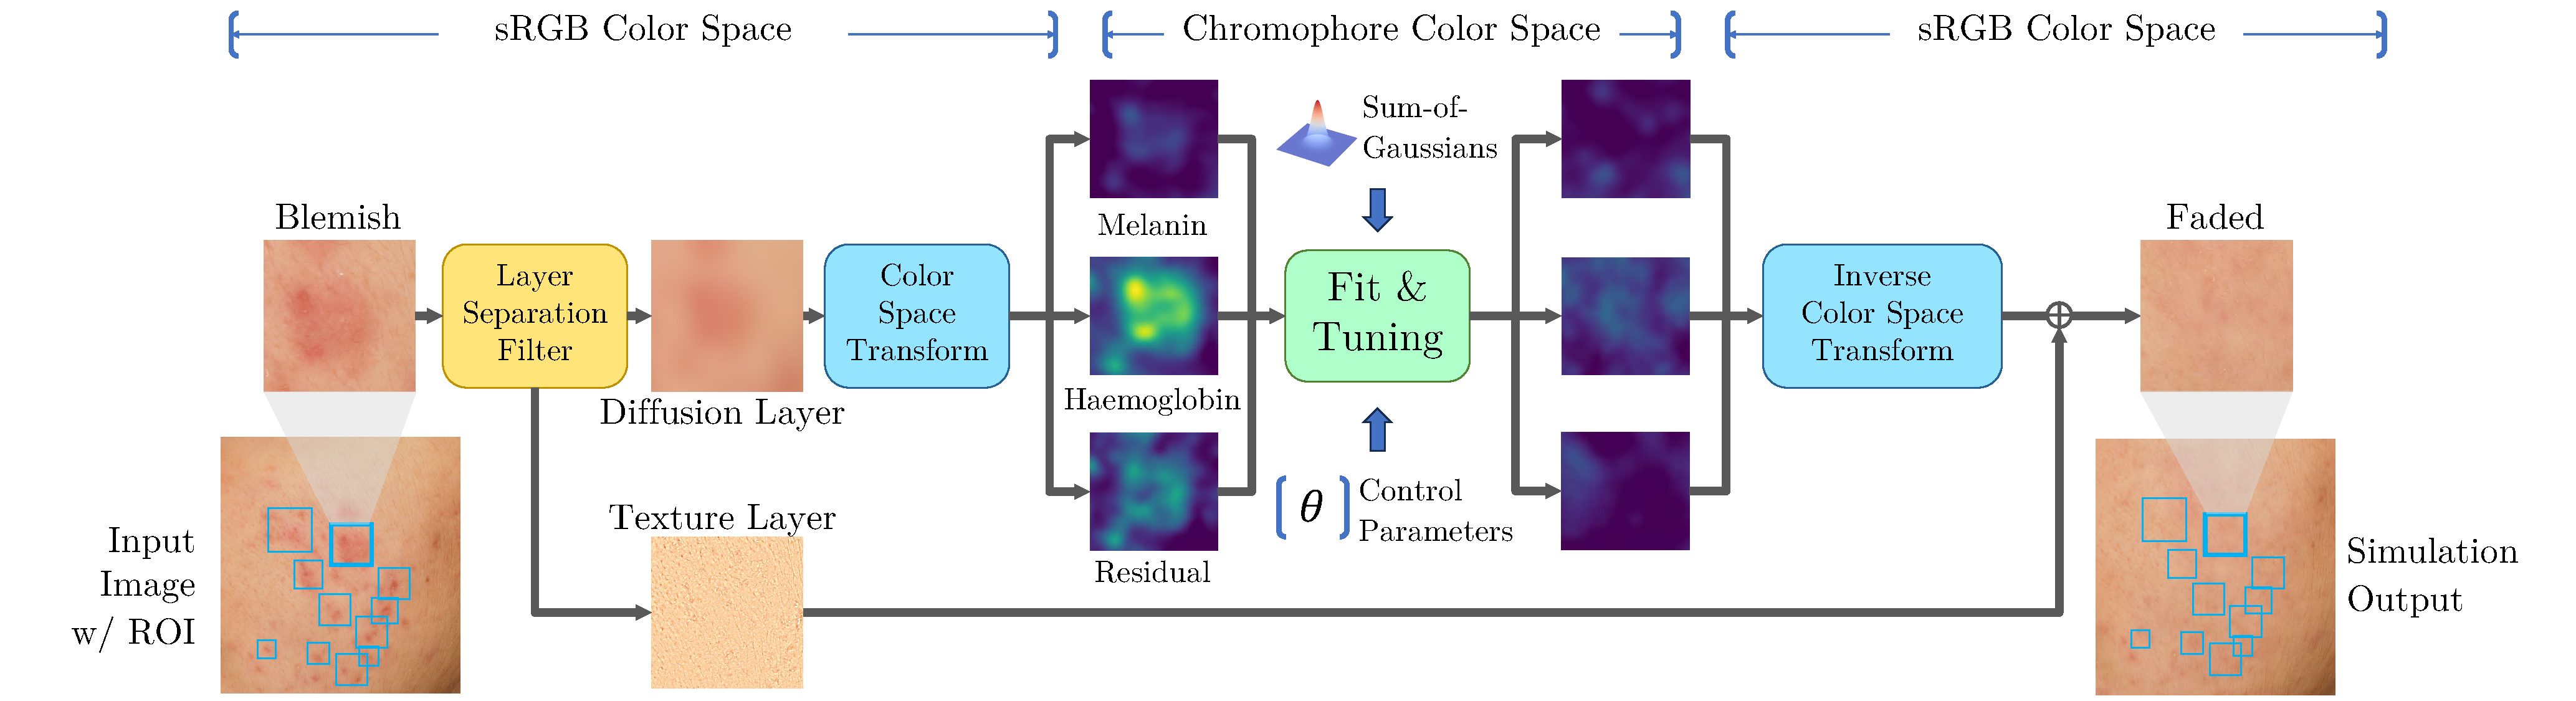
\includegraphics[width=0.94\columnwidth]{Chapter3/system.pdf}
    \caption{An overview of the proposed skin blemish change simulation pipeline. In the pipeline, a box of Region of Interest (ROI) is first used to select the blemish like acne or pigmentation. Then, a \textit{Layer Separation Filter} is applied to separate the texture layer and the diffusion layers. A \textit{Sum-of-Gaussians} model is fitted to each ROI in \textit{Melanin/Heamoglobin} color space, with the parameters of the fitted model adjusted to manipulate the appearance of the blemishes. The modified diffusion layer is summed with the original texture layer to obtain the output.}
    \label{fig:system}
\end{figure}

\section{Skin Chromophore Color Space Decomposition}
In digital photos, skin color represents only a small subset of the sRGB space, due to unique chromophores contained in the skin, such as melanin and heamoglobin, which give the skin a unique and limited color range. However, finding a transformation from sRGB values to the absolute concentration of skin chromophores is challenging, as the sRGB color space is device-agnostic. It also requires calibrating the camera system using pigmentation data in vivo. This issue is bypassed by modeling the \textit{relative} pigment concentration against the base skin, so that the transformed color space can well express the influence of different chromophores on skin color without the need for camera system calibration.

Specifically, the relative absorption of incident light by the chromophore can be described by the Beer-Lambert law, namely:
\begin{equation}
    A(\lambda) = -log(R(\lambda)) = C\epsilon l,
    \label{eq1}
\end{equation}
where $A$ represents absorption, $R$ is the reflection intensity, $\lambda$ is the wavelengths, $C$ is the relative concentration, $\epsilon$ denotes the extinction coefficient of chromophore and $l$ is the mean optical path length.

In this work, the impact of two chromophores on the skin, melanin and heamoglobin, and a residual term, are mainly considered, as shown in Figure \ref{fig:skin_model}. Therefore, $C\epsilon l$ in equation \ref{eq1} expands as
\begin{equation}
    A(\lambda) = C_H\epsilon_H(\lambda)l_H + C_M\epsilon_M(\lambda)l_M + C_r\epsilon_r(\lambda)l_r,
    \label{eq2}
\end{equation}
where subscript $H$, $M$, and $r$ represent heamoglobin, melanin, and residual chromophore, respectively.

Given the distinct absorption and reflection properties of skin chromophores under varying wavelengths of light, the response of each chromophore is considered across the three primary camera pixel channels: Red ($\mathcal{R}$), Green ($\mathcal{G}$), and Blue ($\mathcal{B}$). This consideration leads to the formulation of Equations \ref{eq1} and \ref{eq2}. These equations model the chromophore response in the context of the color channels, providing a foundation for further analysis and image processing within the scope of the proposed method.
\begin{equation}
    \begin{aligned}
         & C_H\epsilon_H^c l_H + C_M\epsilon_M^c l_M + C_r\epsilon_r^c l_r = -log(R^c) \\
         & c\in\{\mathcal{R},\mathcal{G},\mathcal{B}\},
    \end{aligned}
\end{equation}
or in matrix form
\begin{gather*}
    \mathbf{E}\mathbf{c}=-log(\mathbf{k}),\\
    \mathbf{E}=\begin{bmatrix}
        \epsilon_H^\mathcal{R} l_H & \epsilon_M^\mathcal{R} l_M & \epsilon_r^\mathcal{R} l_r \\
        \epsilon_H^\mathcal{G} l_H & \epsilon_M^\mathcal{G} l_M & \epsilon_r^\mathcal{G} l_r \\
        \epsilon_H^\mathcal{B} l_H & \epsilon_M^\mathcal{B} l_M & \epsilon_r^\mathcal{B} l_r
    \end{bmatrix},\
    \mathbf{c}=\begin{bmatrix}C_H \\C_M \\C_r\end{bmatrix},\
    \mathbf{k}=\begin{bmatrix}R^\mathcal{R} \\R^\mathcal{G} \\R^\mathcal{B}\end{bmatrix}.
\end{gather*}

\begin{figure}[t!]
    \centering
    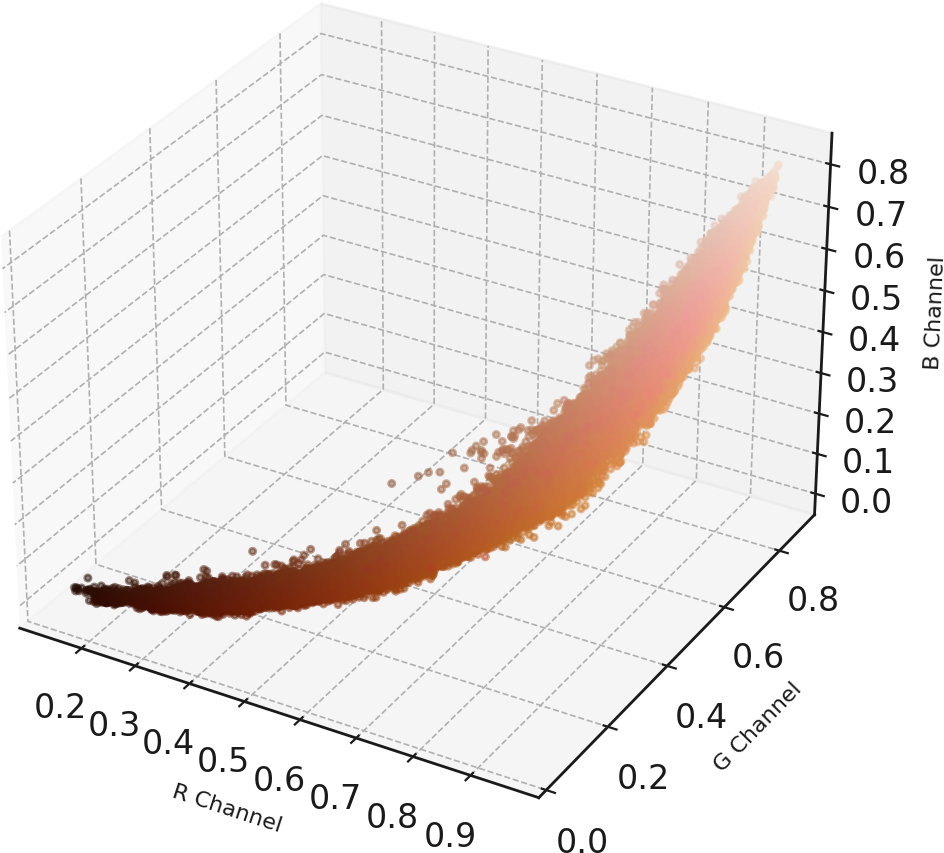
\includegraphics{Chapter3/original_data_rounded_plot.png}
    \caption{3D scatter plot showing the distribution of skin colors sampled from the face skin images in a dataset, illustrating the correlation between the R, G, and B channels.}
    \label{fig:3dplot}
\end{figure}

It is reported that there is no significant difference in skin thickness between human races\cite{Whitmore2000}. In other words, $l$ can be seen as a constant. So $l$ is combined with $\epsilon$ in $\mathbf{E}$. Following the practice of Tsumura et al.\cite{tsumura1999independent}, $E$ is estimated by Fast Independent Component Analysis (FastICA)\cite{HYVARINEN2000411} in the log-RGB domain. Specifically, 128 patches are randomly sampled from each face skin image of the dataset, and each patch is 16x16 pixels in size. Then the average RGB value of each patch is calculated, as illustrated in Figure\ref{fig:3dplot}. The FastICA algorithm in \texttt{sklearn}\cite{scikit-learn} is adopted to estimate the 3 independent components over the log-RGB domain as $\mathbf{E}$. In this work, $\hat{\mathbf{E}}$ is obtained as follows:
\begin{equation}
    \hat{\mathbf{E}} = \begin{bmatrix}
        0.96  & -0.63 & 0.9  \\
        -0.22 & 0.35  & 0.17 \\
        -0.16 & -0.69 & -0.4 \\
    \end{bmatrix}
\end{equation}

\section{Blemishes Appearance Modelling \& Editing}
Given a 3-channel image patch $C(\mathbf{x})\in\mathbb{R}^{3\times h\times w}, \mathbf{x}\in\mathbb{R}^2$ with length $w$ and height $h$, containing a user-selected blemish, it assumes that the patch can be divided into normal skin $C_K^{skin}$ and blemish $C_K^{blem}$ in chromophore color space, that is
\begin{equation}
  C_K(\mathbf{x}) = C_K^{skin}(\mathbf{x}) + C_K^{blem}(\mathbf{x}),\quad K\in\{H,M,r\}.
\end{equation}
For the estimation of $C_K^{skin}$, it assumes that skin color changes are smooth within a local area. Therefore, it can be fitted by a simple linear model
\begin{equation}
  \hat{C_K^{skin}}(\mathbf{x};\mathbf{k},d)=\mathbf{k}\mathbf{x}+d,\quad\mathbf{k}\in\mathbb{R}^2, d\in\mathbb{R}.
\end{equation}
For the estimation of $C_K^{blem}$, the proposed method is based on the observation that pigmentation and acne of interest tend to have blurred edges due to the subsurface scattering of light under the skin. On one hand, they are caused by local accumulation of chromophores under the skin due to various stressors such as UV or inflammation, which can be modeled as Gaussian distributions. On the other hand, subsurface scattering of light under the skin makes blemishes look even blurry. With Gaussian functions, both phenomena can be described very well, because the convolution of two Gaussian functions is still a Gaussian function, namely:
\begin{equation}
    \begin{aligned}
         & G(x; \mu_a, \sigma_a, a)\star G(x; \mu_b, \sigma_b, b)                 \\
         & \qquad= a\cdot b\cdot G(x; \mu_a+\mu_b, \sqrt{\sigma_a^2+\sigma_b^2}),
    \end{aligned}
\end{equation}
where $\star$ is the convolution operator, and Gaussian function $G$ is defined as
\begin{equation}
    G(x; \mu, \sigma, a) = \frac{a}{\sigma\sqrt{2\pi}}e^{-\frac{{(x - \mu)^2}}{{2\sigma^2}}}.
\end{equation}
For multivariate Gaussian functions (2D in this research), they can be denoted as
\begin{equation}
    G(\mathbf{x}; a, \mathbf{\mu}, \Sigma)=\frac{a}{2\pi\sqrt{|\Sigma|}}e^{-\frac{1}{2}(\mathbf{x}-\mathbf{\mu})^T\Sigma^{-1}(\mathbf{x}-\mathbf{\mu})},
  \end{equation}
where $\mathbf{\mu}=[\mu_x,\mu_y]^T$ is the centre coordinate $(x,y)$ on the input image plane, $\Sigma\in\mathbb{R}^{2\times2}$ is the covariance matrix and $a$ is the amplitude factor. And note that the above conclusion can also be generalized to this multivariate case.

To better fit variously shaped blemishes and uneven facial areas, $\Sigma$ can be further decomposed into multiplication of rotation matrix $\mathbf{R}$ and scaling matrix $\mathbf{S}$ as
\begin{equation}
    \Sigma= \mathbf{R}\mathbf{S}\mathbf{S}^T\mathbf{R}^T.
\end{equation}
This allows Gaussian functions to stretch and off-axis rotation with an angle of $\theta\in[0,\pi)$, forming ellipsoidal patterns, that is
\begin{equation}
  \mathbf{R} = \begin{bmatrix}
    \cos\theta & -\sin\theta \\
    \sin\theta & \cos\theta
  \end{bmatrix},\quad\mathbf{S}=diag(\sigma_x,\sigma_y).
\end{equation}
Or explicitly
\begin{equation}
    \begin{aligned}
         & G(x, y; \mu_x, \mu_y, \sigma_x, \sigma_y, \theta, a)\\
         & \qquad=\frac{a}{2\pi \sigma_x \sigma_y}\cdot e^{-\frac{{x''^2}}{{2 \sigma_x^2}} - \frac{{y''^2}}{{2 \sigma_y^2}}},\ where \\
         & x'=x - \mu_x, \quad y'=y - \mu_y, \\
         & x'' = x' \cos\theta - y' \sin\theta,\quad y'' = x' \sin\theta + y' \cos\theta.
    \end{aligned}
\end{equation}
Finally, following the existing fast subsurface scattering implementations, the appearance of a blemish under the scattering skin tissue is approximated by sum of multiple Gaussian functions. That is, the estimated distribution $\hat{C_K^{blem}}(\mathbf{x})$ can be denoted by
\begin{equation}
  % \begin{aligned}
  \hat{C_K^{blem}}(\mathbf{x}; \Theta)=\sum_{i=0}^{N-1}G_i(\mathbf{x}; \Theta_i),\ N\ge1, \Theta_i=\left[a_i, \mathbf{S}_i, \mathbf{\mu}_i, \theta_i\right].
  % \end{aligned}
\end{equation}
The parameters are fitted by the Levenberg-Marquardt method\cite{10.1007/BFb0067700} with the \texttt{lmfit} Python library\cite{newville_matthew_2014_11813}. After successful fitting, $\hat{C_K^{skin}}$ is discarded. Instead, $\hat{C_K^{blem}}$ is multiplied with a user-input gain $\alpha_K\in\mathbb{R}$ and add it with the input $C_K(\mathbf{x})$ to amplify/attenuate the blemish intensity to obtain the modified image patch $C_K^{\prime}$, namely
\begin{equation}
  C_K^{\prime} = C_K+\alpha_K\hat{C_K^{blem}}.
  \label{eqn:alpha}
\end{equation}
Obviously, if $\alpha_K=-1$, the facial blemish will be completely removed from the image patch, while a positive gain will intensify this blemish.

\subsection{Algorithm Implementations}
\subsubsection{Preporcessing}
% As shown in Figure \ref{fig:system}, in the pipeline, a skin layer separation filter is first adopted to separate the skin into a surface texture layer (including specular reflections and skin textures) and a scattered chromophore layer. This is implemented using a Gaussian filter with a small variance, small enough to isolate the detail texture of the skin without affecting the underlying assumptions.
In the proposed methodology, as depicted in Figure \ref{fig:system}, the primary focus is laid on the \textit{Diffusion Layer} of the image. To isolate this layer, a skin layer separation filter is first adopted to separate the skin into a surface \textit{Texture Layer} (including specular reflections and skin textures) and a \textit{Diffusion Layer}. This is implemented using a Gaussian filter with a small variance, small enough to isolate the detail texture of the skin without affecting the underlying assumptions. 

Subsequently, in color space transform stage, inverse gamma correction is applied to the standard RGB (sRGB) image to derive linear RGB values. These values are then converted to their logarithmic form, representing an approximation of the real reflectance values, denoted as $R$ in Equation\ref{eq1}. While this approximation may not perfectly mirror the actual scenario, it proves adequate for estimating the relative concentration ratio in comparison to the surrounding skin.
\subsubsection{Optimizations in Fitting Process}
In the actual implementation, several optimizations are performed to the program:
\begin{itemize}
    \item Each channel and each blemish can be fitted independently and multi-process parallelism can be used to speed this up. Thus, the program packages each fitting session into a task and uses Python's thread pool to build a task queue, fully utilizing the computing power of multi-core CPUs.  
    \item Although the entire Sum-of-Gaussians model could be fitted at once, the convergence of the fit would be slow. Therefore, a strategy is adopted where a new $N$-th Gaussian function is gradually introduced into the model with $N-1$ functions and the updated model is fitted, during which the existing parameters are frozen. Finally, all parameters are unfrozen for one more fitting as a fine-tuning. In this way, only one function is fitted each time except for the last one.
    \item In Levenberg-Marquardt iterations, it requires compute the Jacobian matrix for each steps. Since each component in $\hat{C_k}$ has explicit partial derivatives and they are just simply summed togeter, the Jacobian matrix of $\hat{C_k}$ can be manually derived. This assists the Levenberg-Marquardt algorithm to quickly compute accurate gradients rather than estimate them numerically.
\end{itemize}
This algorithm can be represented by the following pseudocode.
\begin{algorithm}
    \caption{Fitting Distribution of a Blemish}
    \begin{algorithmic}[1]
    
    \State \textbf{Input:} Blemish image patch $X\in\mathbb{R}^{3\times h \times w}$, per-channel gain $\alpha_K\in\mathbb{R}^3$. All from user-input.
    
    \State \textbf{Preprocessing:}
    % \Indent
        \State $X_d, X_t \gets GaussianFilter(X)$ \Comment{$X_d$:Diffusion Layer, $X_t$:Texture Layer}
        \State $X_d \gets \gamma^{-1}(X_d/255.0)$ \Comment{Inverse gamma transformation to linear RGB space}
        \State $X_d \gets \mathbf{E}^{-1}\cdot\log{X_d}$ \Comment{Transform to chromophore color space}
    \For{each channel $k \in \{H, M, r\}$ of $X_d$}
        \State Initialize linear normal skin model $\hat{C_k}\gets\hat{C_k^{skin}}$
        \For{each Gaussian component $G^i_k$}
            % \State Estimate initial center position $x^{init}_i, y^{init}_i$
            \State Fit $G_k^i(x, y; \mu_x^i, \mu_y^i, \sigma_x^i, \sigma_y^i, \theta^i, a^i)$
            \State $\hat{C_k} \gets \hat{C_k}+G_k^i$
            \State Freeze parameters of $\hat{C_k}$
        \EndFor
        \State Unfreeze all parameters for final refinement fit
        \State $\hat{C_k} \gets \alpha_k\cdot(\hat{C_k}-\hat{C_k^{skin}})$
    \EndFor
    \State $X_d \gets X_d+\hat{C_k}$
    \State $X_d \gets InverseColorTransform(X_d)$
    \State $X \gets X_d+X_t$
    \State \textbf{Return:} Fitted parameters and modified blemish image
    \end{algorithmic}
    \end{algorithm}

\begin{figure}[t!]
    \centering
    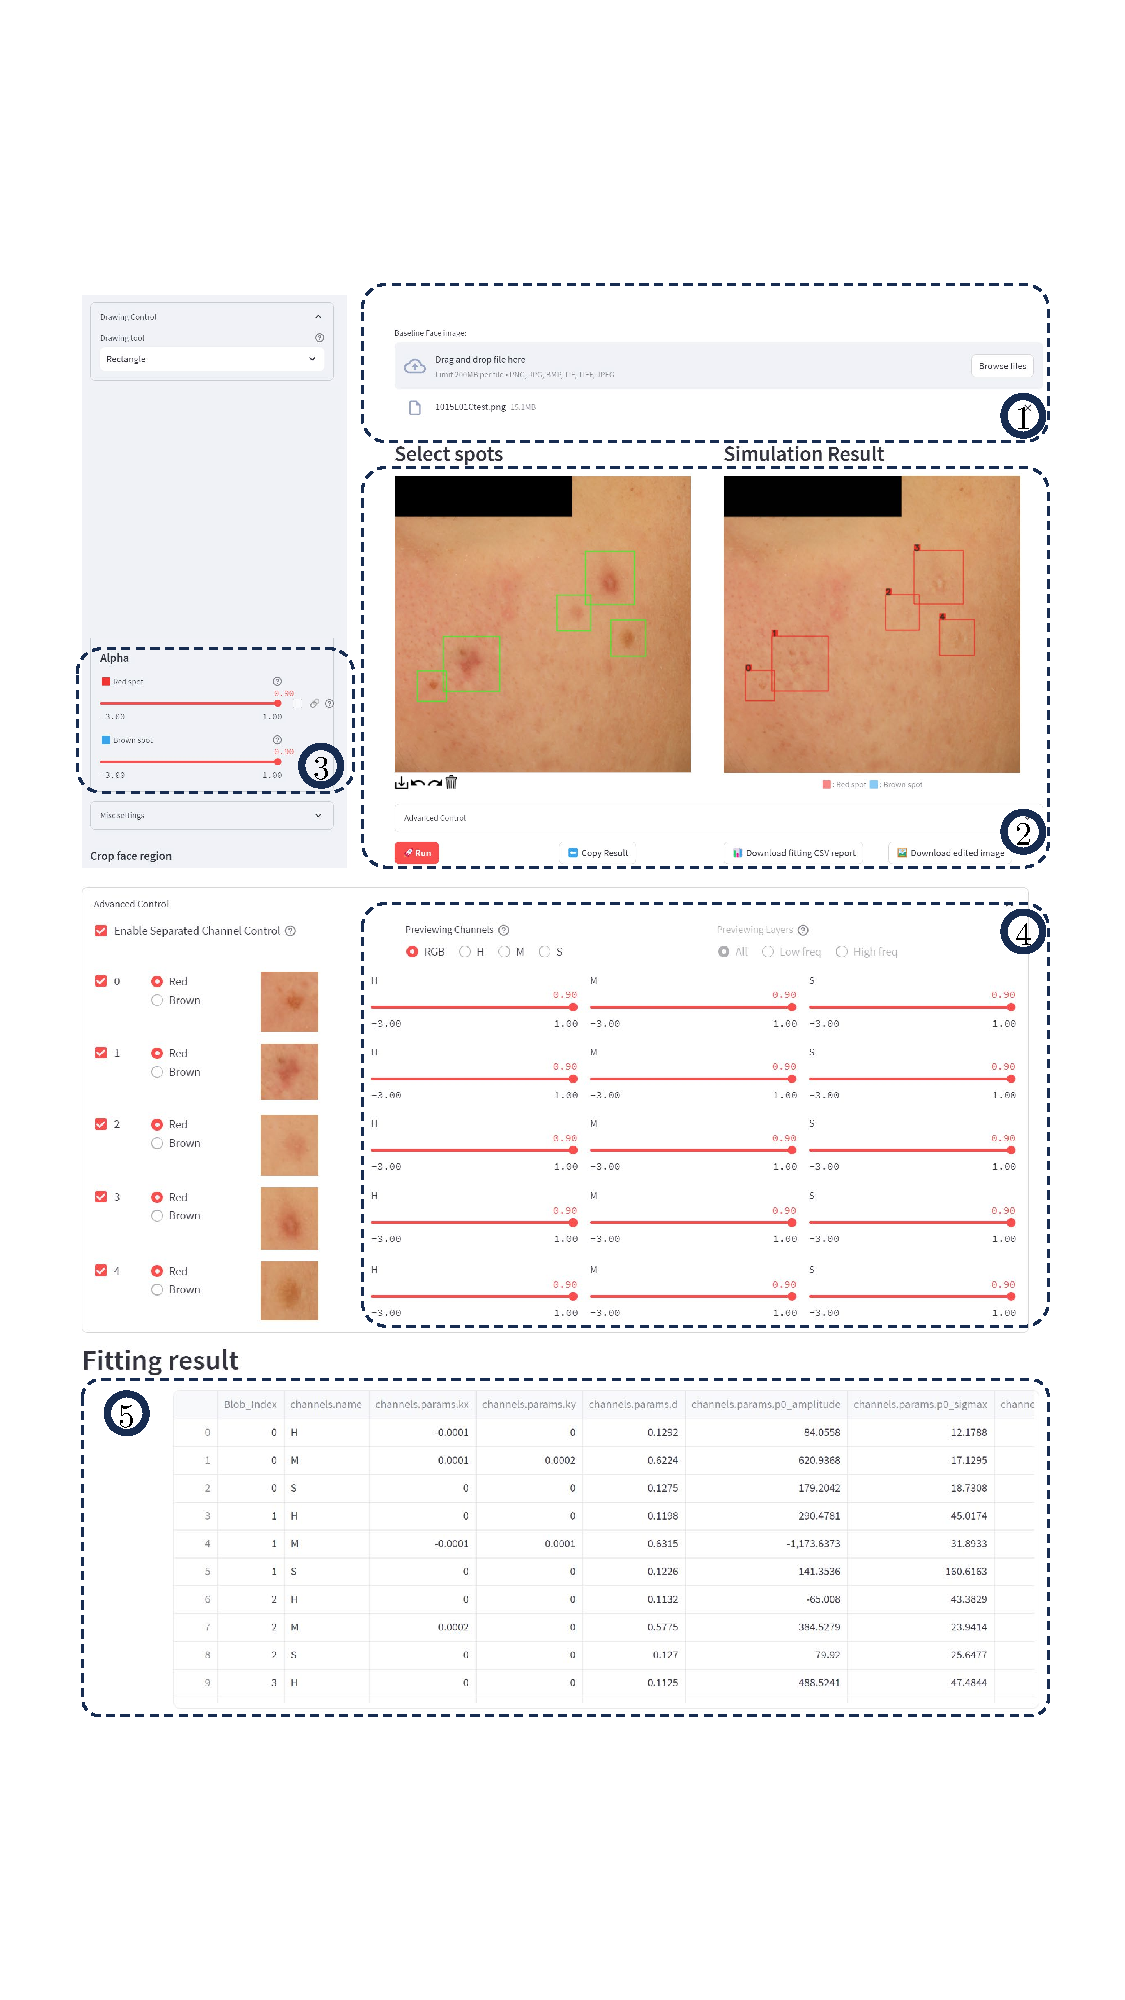
\includegraphics[width=0.93\columnwidth]{Chapter3/GUI.pdf}
    \caption{An Overview of GUI}
    \label{fig:gui}
\end{figure}
\subsubsection{GUI Implementations}
\vspace{-1.2em}
As shown in Figure\ref{fig:gui}, a simple graphical user interface (GUI) is also created to facilitate the editing of facial images by users with varying levels of expertise. The GUI is organized into several sections, each providing tools for specific tasks in the editing process.
\begin{itemize}
    \item \textbf{Image Upload and Blemish Selection} The initial interaction with the interface is the image upload functionality, denoted by circled numeral 1 in Figure \ref{fig:gui}. Users can upload the facial image they intend to edit. Following the upload, the image is displayed within the central work area of the GUI, allowing users to identify and select skin blemishes for removal or modification. This selection process is designed to be intuitive, employing a simple point-and-click mechanism to mark areas of interest, as indicated by circled numeral 2.
    \item \textbf{Basic and Advanced Editing Controls} After blemish selection, users can adjust the editing intensity using the 'alpha' parameter, a slider control located in the section marked by circled numeral 3 in Figure \ref{fig:gui}. This allows for the manipulation of the editing gain in a user-friendly manner. Activating the 'Run' button initiates the rendering process, culminating in the display of the modified image where the selected blemishes have been processed according to the specified parameters.

    For users requiring more sophisticated control, the interface offers advanced editing options as shown in circled numeral 4. This advanced control panel permits individual adjustments to the gains of separate color channels, thus affording an enhanced level of precision in the blemish editing process.
    \item \textbf{Parameter Exportation for Analysis} An essential feature of the GUI, highlighted in circled numeral 5 in Figure \ref{fig:gui}, is the ability to download the fitting results. This function caters to expert users who wish to perform a detailed analysis of the editing parameters or to utilize these parameters for further processing steps, thereby extending the capabilities of the system.
\end{itemize}
%=== END OF CHAPTER THREE ===
\end{spacing}
\newpage

%=== CHAPTER FOUR (4) ===
%=== Test and Experiments ===

\chapter{Experiments}
\begin{spacing}{1.5}
\setlength{\parskip}{0.3in}
\section{Dataset}
To the best of the authors' knowledge, there is currently no dataset for studies of skin blemish modification and fading. Therefore, a self-collected dataset is adopted for research, development, and testing. The images within the dataset were acquired by two clinical imaging systems (Visia CR4 and OLE, both developed by Canfield Scientific). They were cross-polarized and color-calibrated and had a minimum resolution of $3700 \times 5600$. The dataset consists of 223 subjects within the age range of 18 to 45 years, encompassing multi-ethnic consumers with skin tones ranging from dark to light, quantitatively assessed using the Individual Typology Angle (ITA), visualized in Figure \ref{fig:ita}. The ITA for each subject is calculated using the formula:
\begin{equation}
\text{ITA} = \arctan\left(\frac{L* - 50}{b*}\right) \times \frac{180}{\pi},
\end{equation}
where $L*$ and $b*$ are coordinates from the CIE-LAB color space representing the lightness and the chromaticity on the yellow/blue axis, respectively. This measure provides a valuable tool for analyzing skin tone diversity in the dataset. The collection period lasted for a duration of up to 3 months during the Summer season with a time step of one week. The summary of the dataset is shown in Table \ref{tbl:dataset_summary}. In the simulation, images of Week 0 are input and the parameters of the obtained model are adjusted to simulate the change of the blemishes in the following weeks. As shown in Figure\ref{fig:forward}, the input is labelled as \textit{Week 0} and the images for the next few weeks as \textit{+n W}.

\begin{table}[t!]
    \caption{Summary of Dataset Statistics}
    \resizebox{\columnwidth}{!}{%
    \begin{tabular}{lrlrlr}
        \toprule
        \multicolumn{2}{c}{\textbf{ITA Score}} & \multicolumn{2}{c}{\textbf{Ethnicity}} & \multicolumn{2}{c}{\textbf{Skin Tone Classification}} \\
        \midrule
        \midrule
        Total Subjects        & 223   & African       & 126 & Dark         & 76 \\
        ITA Mean              & 2.58  & Caucasian     & 98  & Brown          & 132  \\
        ITA Variance          & 851.90 & Indian       & 108 & Tan           & 152 \\
                              &       & Latino        & 114 & Intermediate  & 62 \\
                              &       &               &     & Light         & 8   \\
        \bottomrule
    \end{tabular}
    }
    \label{tbl:dataset_summary}
\end{table}
\begin{figure}[t!]
    \centering
    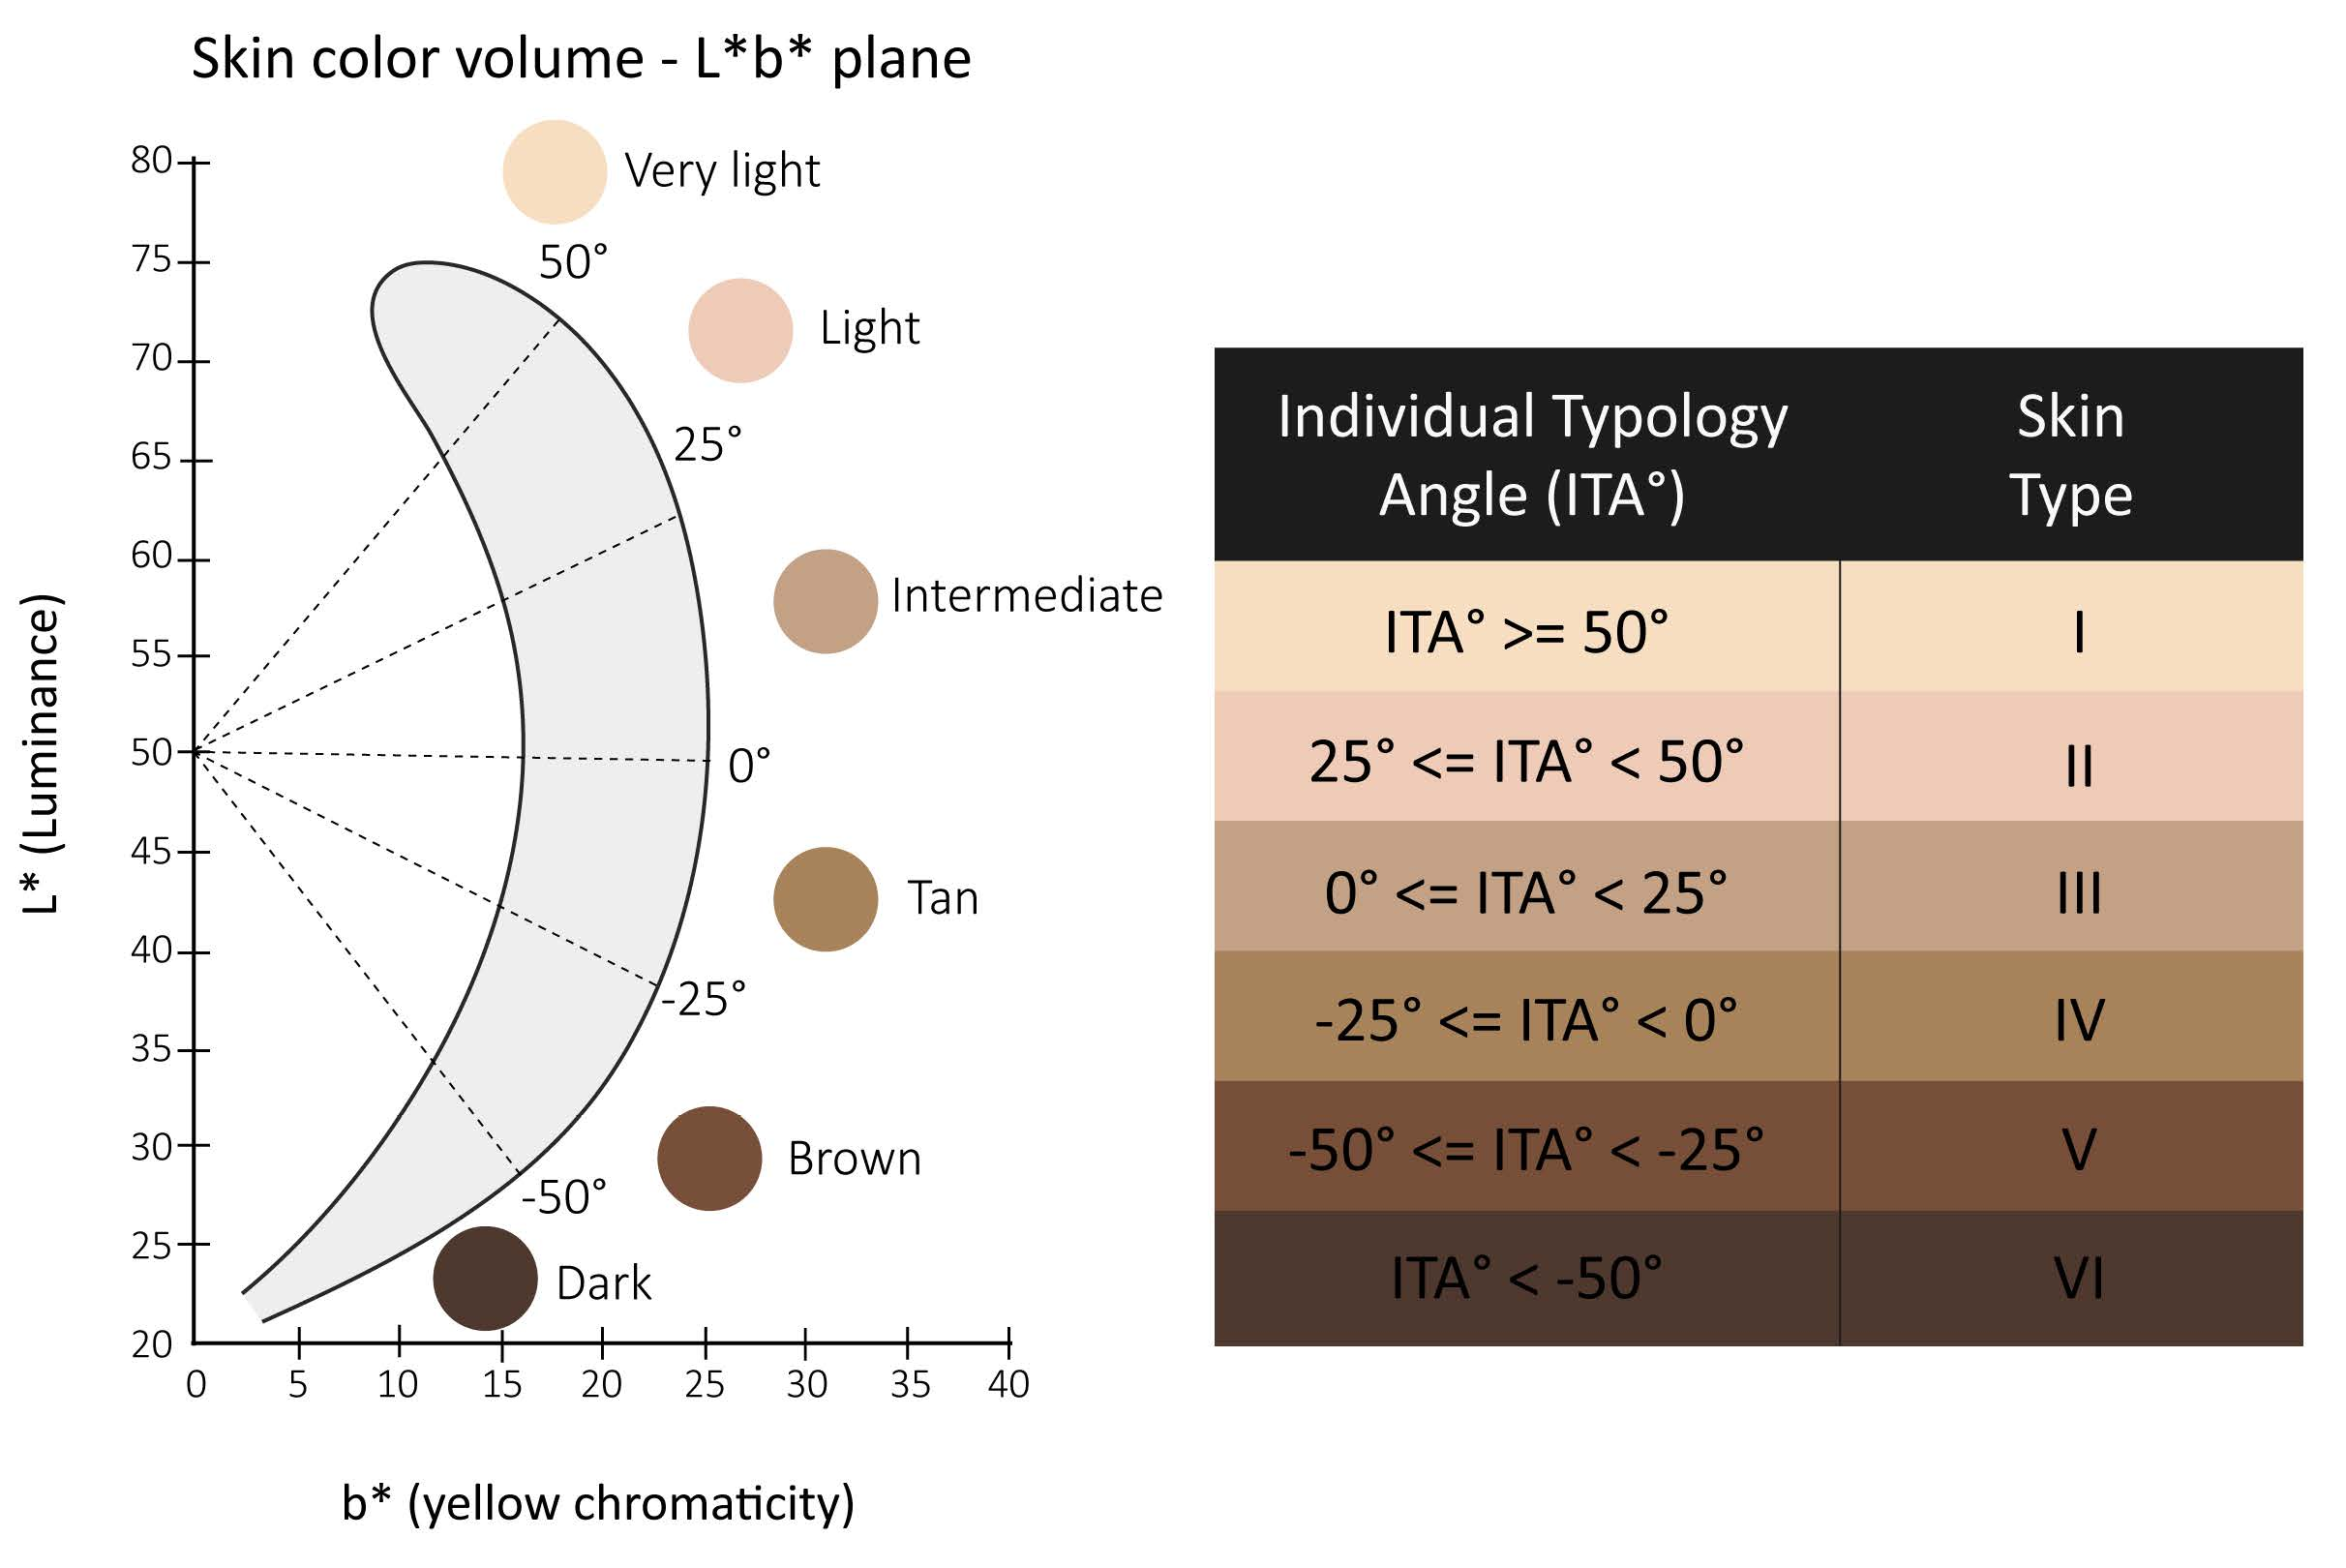
\includegraphics[width=0.97\columnwidth]{Chapter4/ITA.jpg}
    \caption{Visualisation of ITA classification threshold within the L* and b* color space, used for determining skin tone categories. The left side shows the skin color volume on the L*-b* plane with indicative angles for various skin tones, while the right side presents specific ITA ranges with corresponding skin rone classifications from I (very light) to VI (dark). Our dataset encompasses a diverse spectrum of skin tones, including categories from dark (Skin Type VI) to light (Skin Type II). Image taken from \cite{krishnapriyaAnalysisManualAutomated2022a}.}
    \label{fig:ita}
\end{figure}

\section{Experiment Setup}
In this study, extensive blemish change simulation experiments are carried out to evaluate the proposed algorithm's effectiveness. Each blemishes is fitted with 3 Gaussian functions summation and $\sigma=10$ is set for the skin texture layer separation filter. The focus is mainly on the relative concentration changes of the blemishes, and a series of simulations are conducted based on tuning the concentration parameter after successfully fitting blemishes.

Inpainting mode of \textbf{Stable Diffusion}(SD)\cite{rombach2021highresolution} and \textbf{Adobe Photoshop}(PS)'s inpainting tool\cite{adobephotoshop} are selected for comparison as baseline models, as shown in Figure \ref{fig:ps_sd}. The former, a top-performing deep learning model, represents the "latent space editing" method discussed. For the SD method, the inpainting mode is used and the text prompt is set as \texttt{skin patch, human face skin, high definition, best quality}, as shown in Figure \ref{fig:sd}. Each test is performed with 50 iterations of sampling using the \texttt{DPM++SDE Karras} sampler, with the random seed fixed to 42. The denoising ratio is adjusted to increase the difference between the generated image and the original so that the intensity of blemish removal is controlled. 

For the PS method, a common image editing software, represents the "pixel space editing" method. Here, the inpainting tool is utilized, selecting and removing blemishes on the original image with \textit{Content-Aware} mode, as shown in Figure \ref{fig:ps}. The modified image is then combined with the original image through Alpha blending. And the degree of blemish removal is adjusted by altering blending opacity.

\begin{figure}[t!]
    \centering
    \begin{subfigure}{.97\textwidth}
        \centering
        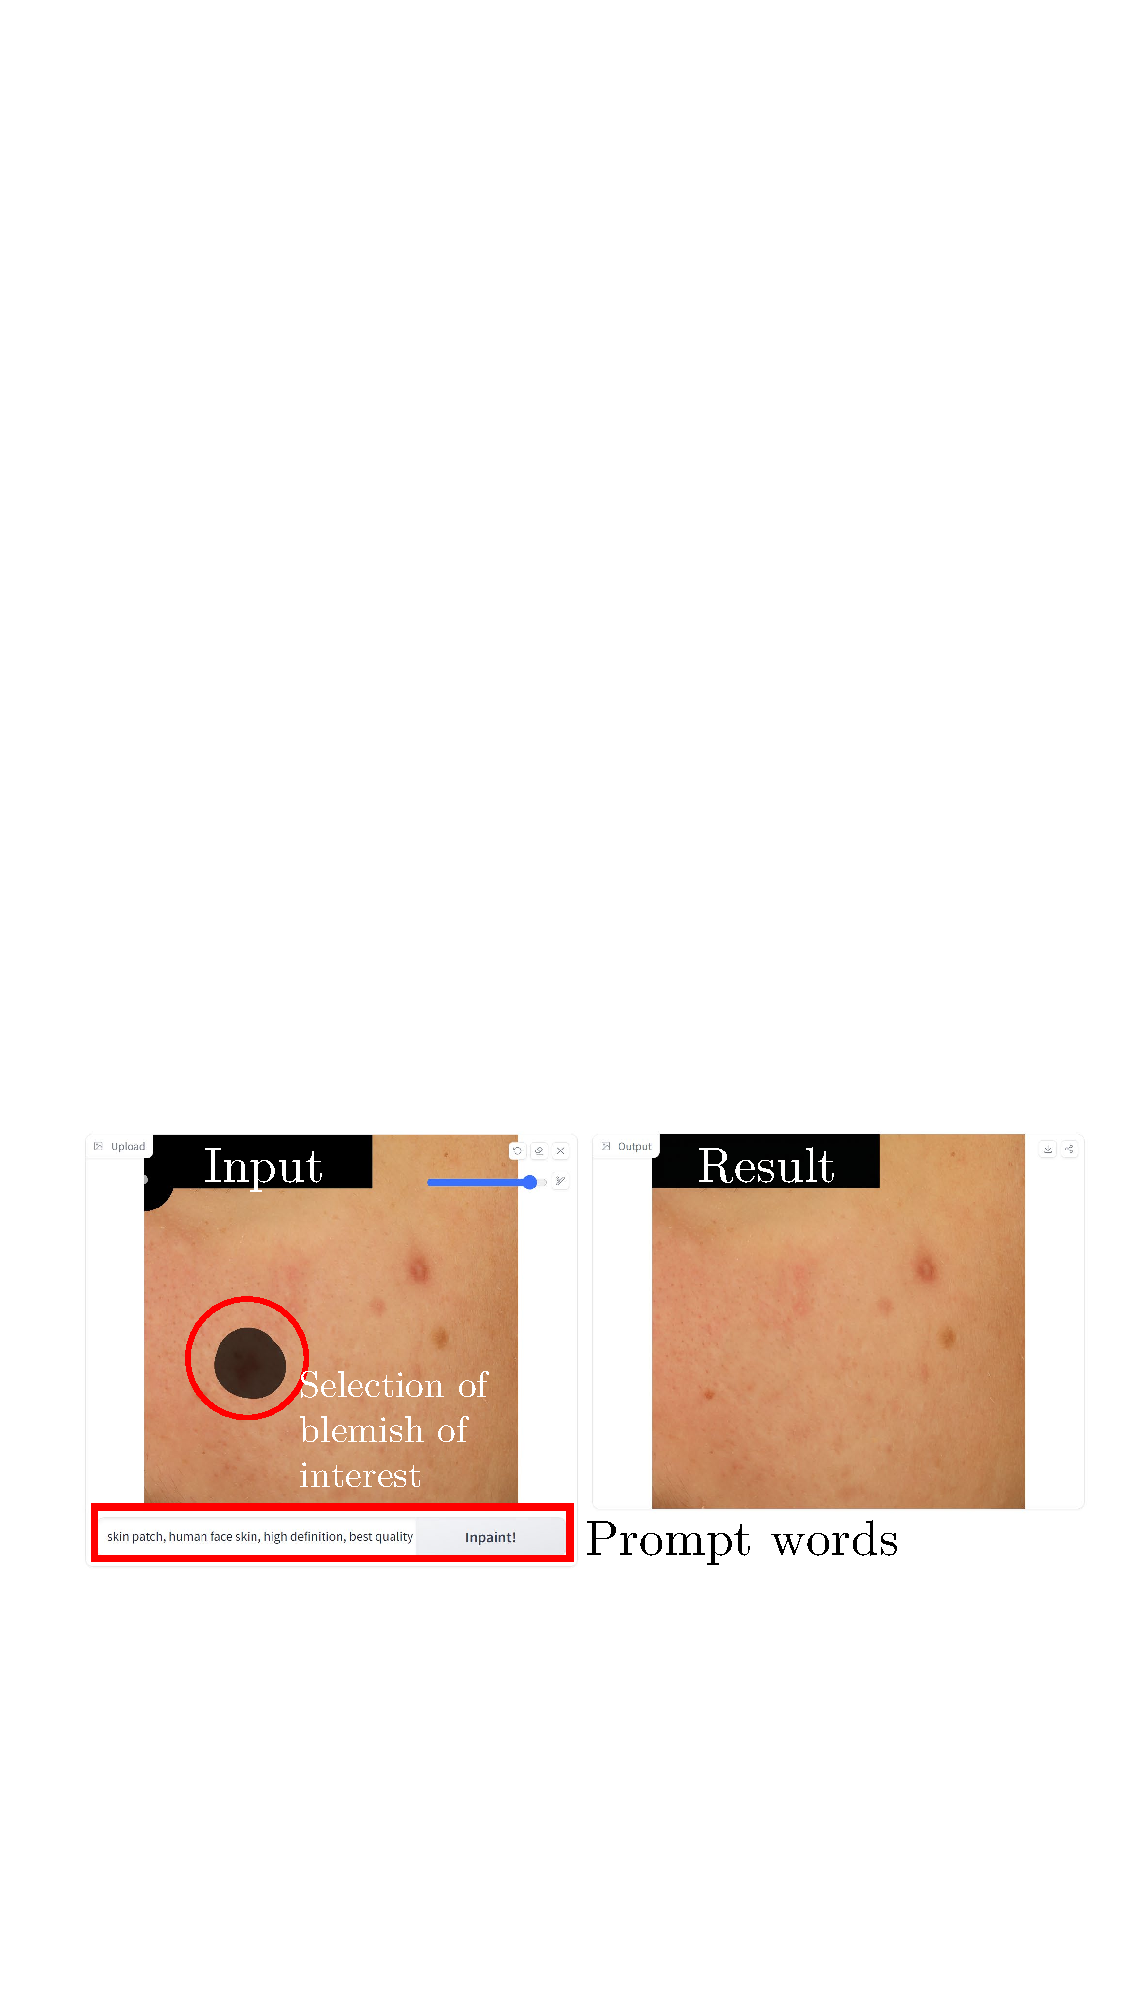
\includegraphics[width=0.97\columnwidth]{Chapter4/sd_ui.pdf}
        \caption{Stable Diffusion (SD) inpainting mode}
        \label{fig:sd}
    \end{subfigure}\hfill
    \begin{subfigure}{.97\textwidth}
        \centering
        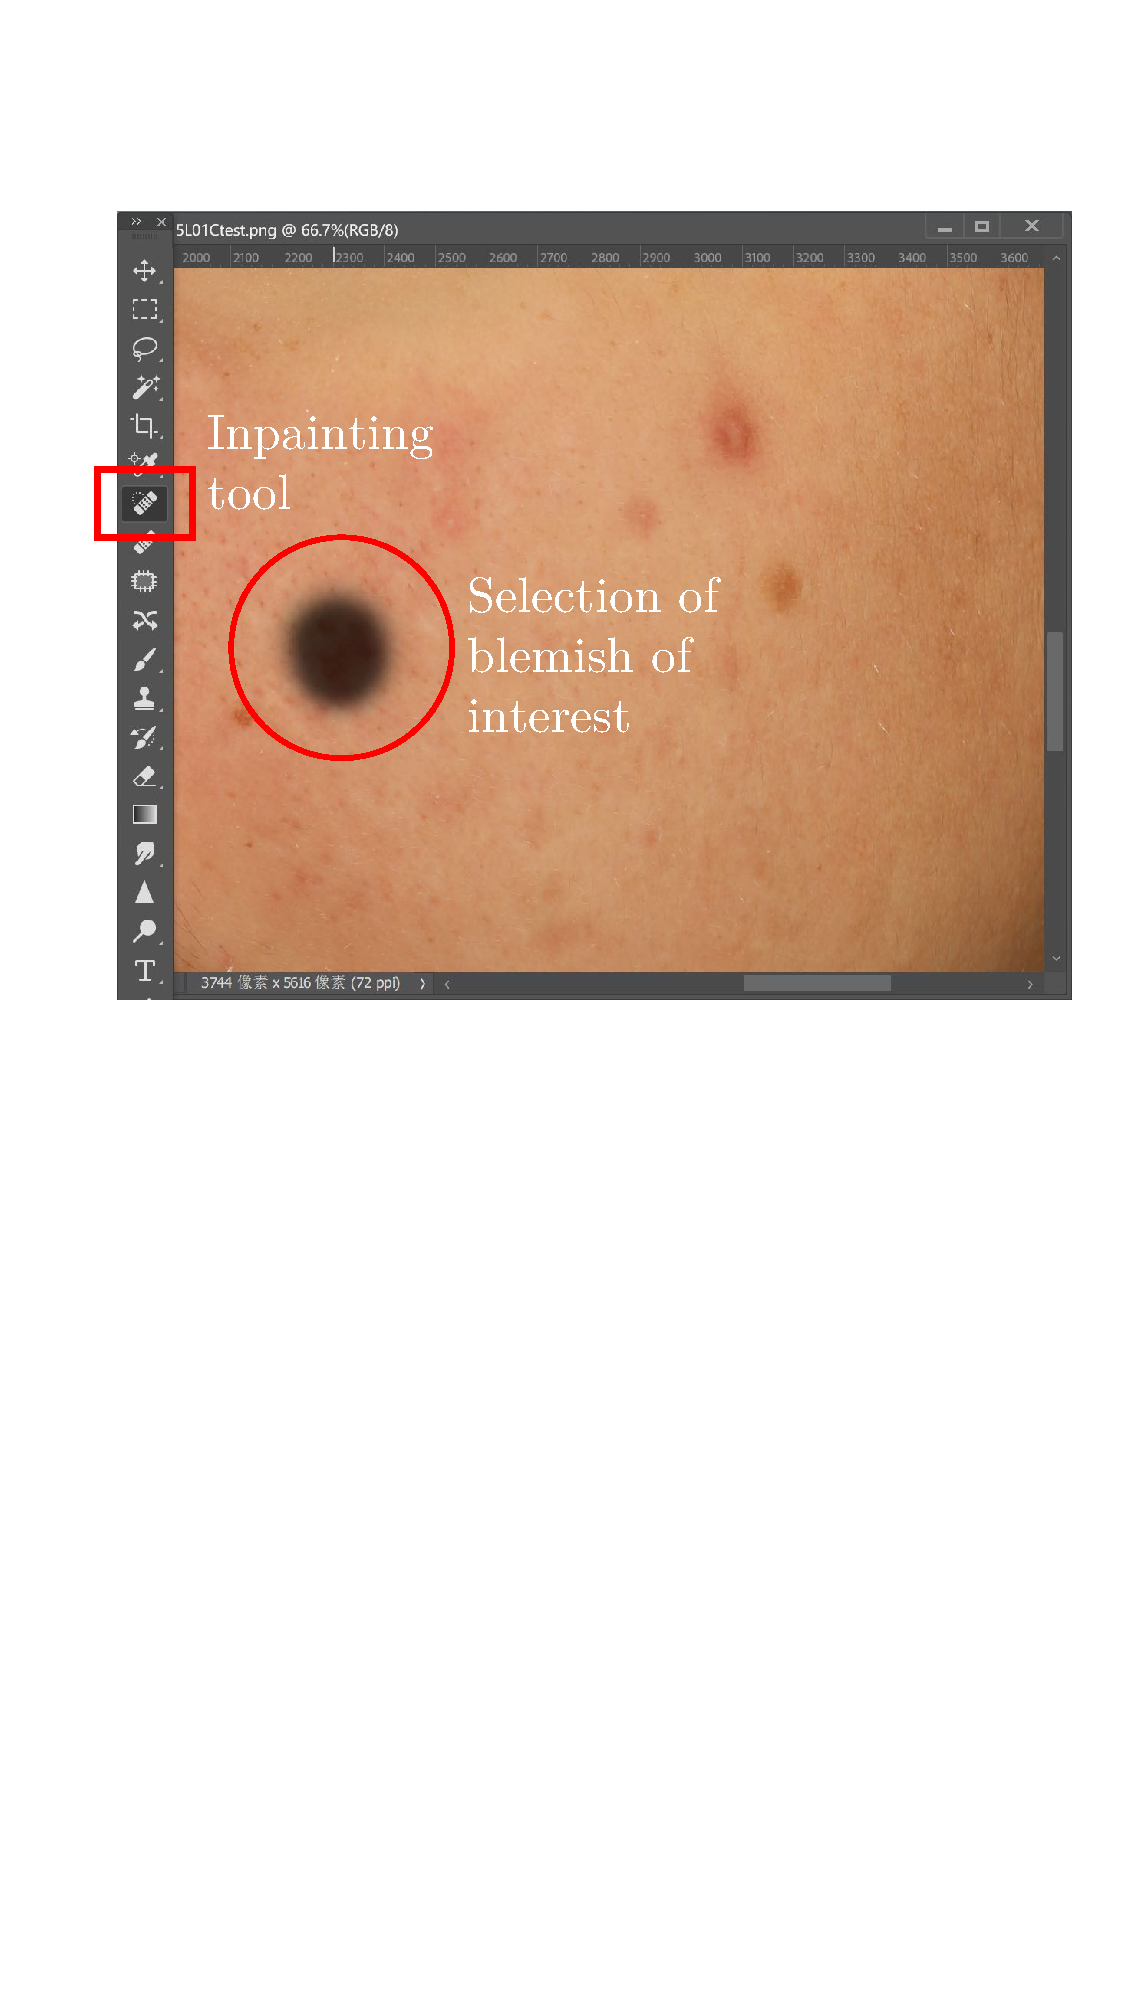
\includegraphics[width=0.97\columnwidth]{Chapter4/ps_ui.pdf}
        \caption{Adobe Photoshop (PS) inpainting tool}
        \label{fig:ps}
        % \label{fig:gui1}
    \end{subfigure}
    \caption{Example of a baseline models. Widely available and easily reproducible baseline methods are selected for comparison. Specifically, Adobe Photoshop(PS) is chosen For \textit{pixel space} editing methods, which is the most commonly used image editing and retouching software. For \textit{latent space} editing methods, Stable Diffusion(SD), recognised for its high-quality generation, is selected.}
    \label{fig:ps_sd}
\end{figure}

\subsection{Objective Evaluation}
To objectively evaluate image modifications, the Fréchet Inception Distance (FID) is applied. FID is a common tool for assessing GANs and similar image-generating models. It uses the Inception V3\cite{DBLP:conf/cvpr/SzegedyVISW16} model to derive the mean and covariance matrix of feature vectors from both authentic and generated image collections. Then, it calculates the Fréchet distance between these statistical groups. This distance gauges the variation between two multi-dimensional Gaussian distributions. Generated images resembling real images more closely have lower FID scores, while higher scores show a bigger divergence. Formally, the FID score is denoted as:
\begin{equation}
    \text{FID} = \|\mu_r - \mu_g\|^2 + \text{Tr}(\Sigma_r + \Sigma_g - 2(\Sigma_r\Sigma_g)^{1/2}),
\end{equation}
where $\mu_r, \mu_g$ represent the mean feature vectors of the real and generated/modified images, respectively. $\Sigma_r, \Sigma_g$ are the covariance matrices of the real and generated/modified images, respectively. And $\text{Tr}(\cdot)$ is the trace of a matrix, which is the sum of the diagonal elements.
% TODO
\subsection{Subjective Evaluation}
To subjectively evaluate the performance of the proposed facial skin blemish simulation algorithm, a visual perception study is conducted. The aim is to comprehensively evaluate whether the proposed algorithm could produce authentic and believable blemish changes and to analyse whether there are biases in certain attributes of the skin, such as skin color or age. A group of 500 panellists join this study, whose age groups are divided into three categories: 19-25; 26-34; and 35-45, covering various ethnicities including Caucasians, African-Americans, Asians, Hispanics, and others, as shown in Figure \ref{fig:metadata}.
\begin{figure}[t!]
    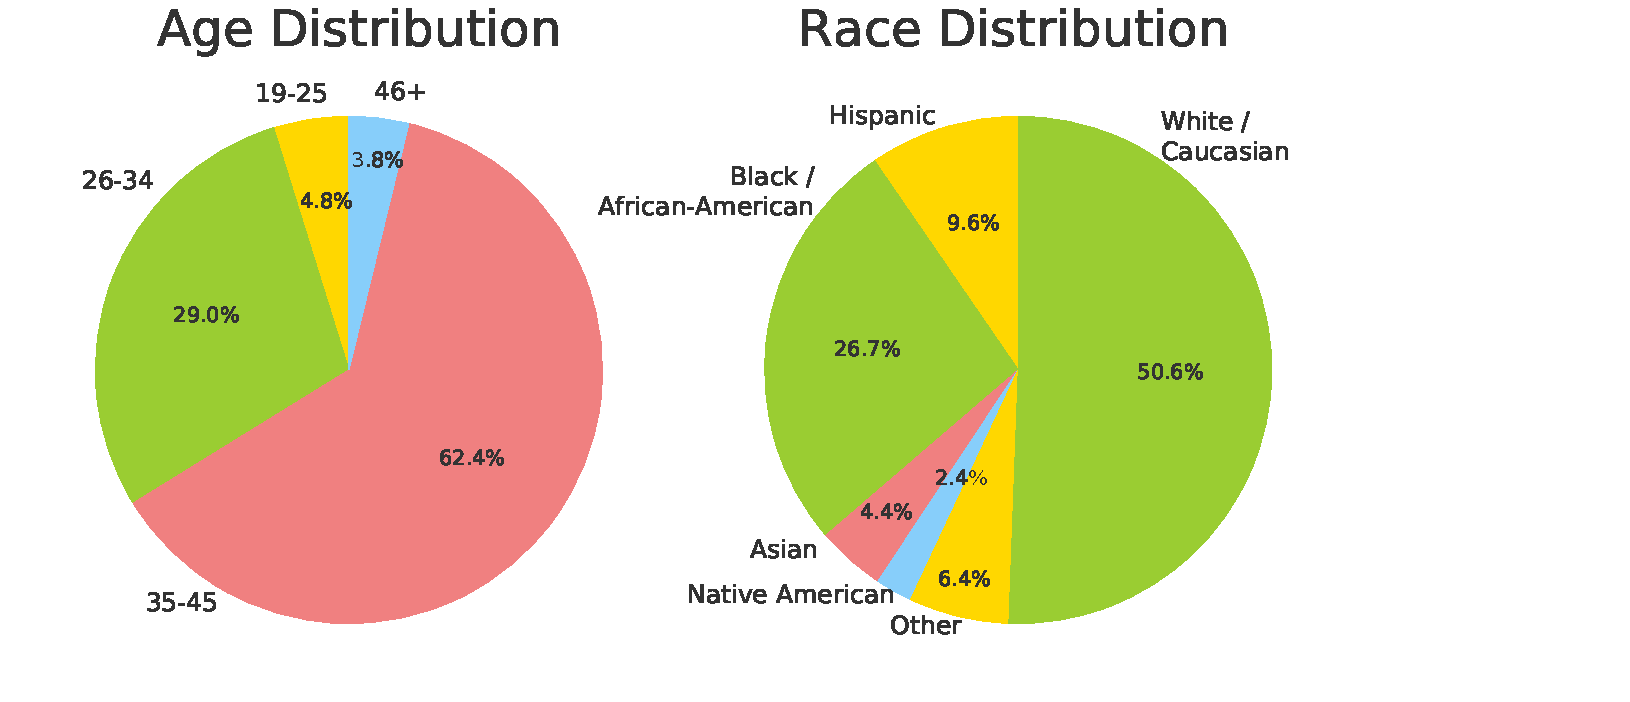
\includegraphics[width=0.95\columnwidth]{Chapter4/metadata.pdf}
    \caption{Metadata of panellists. The test population covers people from 19 to 45 years old, multiple races, and multiple skin tones}
    \label{fig:metadata}
\end{figure} 
\begin{figure}[t!]
    \centering
    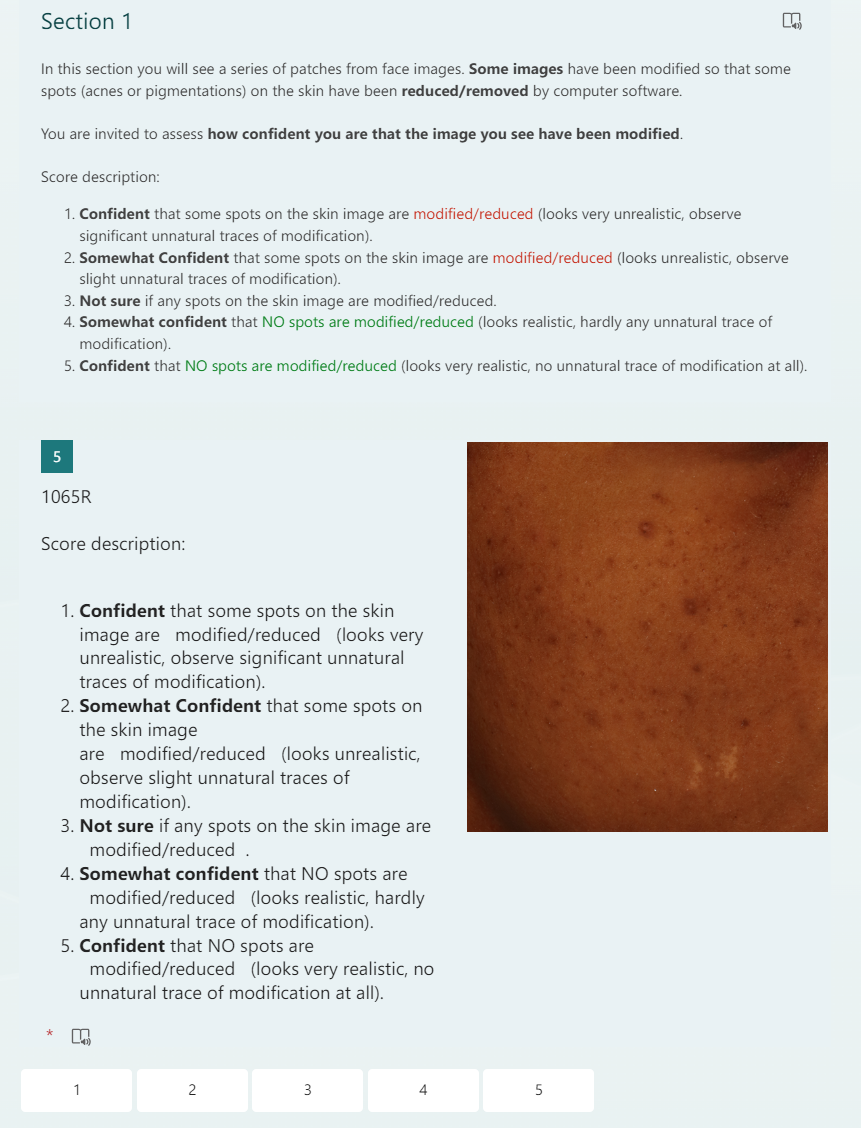
\includegraphics[width=0.9\columnwidth]{Chapter4/sample_form1.png}
    \caption{Examples of questions in the questionnaire. 48 questions of such question are designed, with 24 featuring modified images. For each panellist, 10 questions are randomly selected from the question bank.}
    \label{fig:sample_form}
\end{figure}
In the survey, the question asked is \textit{you will see a series of patches from face images. Some images have been modified so that some spots (acnes or pigmentations) on the skin have been reduced/removed by computer software. You are invited to assess how confident you are that the image you see have been modified.} The answer options are set as:
\begin{itemize}
    \item Confident that some spots on the skin image are modified/reduced (looks very unrealistic, observe significant unnatural traces of modification). (-2)
    \item Somewhat Confident that some spots on the skin image are modified/reduced (looks unrealistic, observe slight unnatural traces of modification). (-1)
    \item Not sure if any spots on the skin image are modified/reduced. (0)
    \item Somewhat confident that NO spots are modified/reduced (looks realistic, hardly any unnatural trace of modification). (+1)
    \item Confident that NO spots are modified/reduced (looks very realistic, no unnatural trace of modification at all). (+2)
\end{itemize}

In the survey, 48 images (24 simulated through the proposed algorithm and 24 unaltered images) are shown to the panellists one image at a time. When the score ranges from 0 to +2, the respondents are considered to be affirming the image as "real" rather than modified. A sample question in the survey is shown as Figure \ref{fig:sample_form}.
%=== END OF CHAPTER FOUR ===
\end{spacing}
\newpage

%=== CHAPTER FIVE (5) ===
%=== Discussion ===

\chapter{Result \& Discussion}
\begin{spacing}{1.5}
\setlength{\parskip}{0.3in}
\begin{figure}[h]
    \centering
    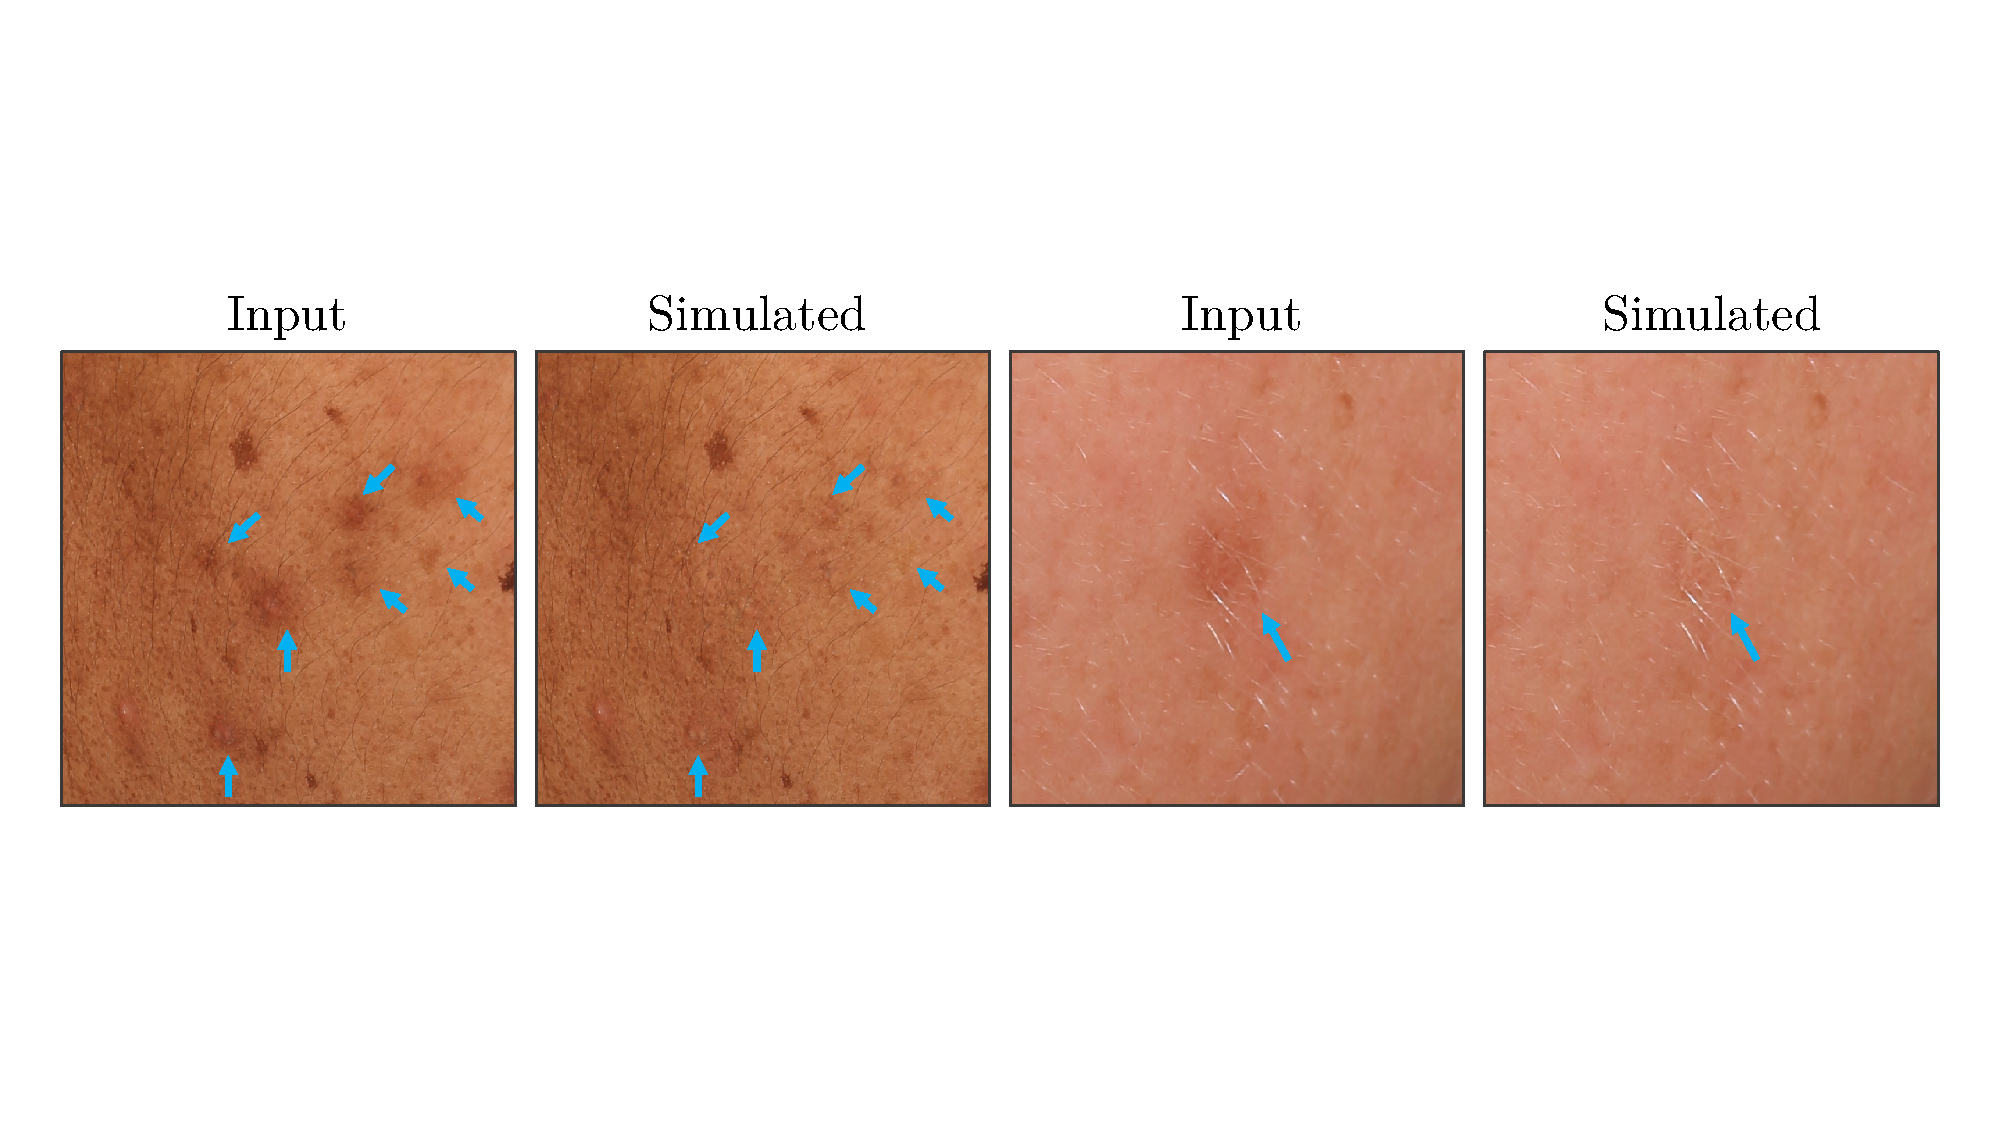
\includegraphics[width=0.9\linewidth]{Chapter5/img_comp2.pdf}
    \caption{Zoomed-in detail of the blemish fading simulation results. Blue Arrows are manually added to highlight blemishes of interest (acne or pigmentation). Note that the proposed method keeps skin details (e.g., hairs, texture) unaltered.}
    \label{fig:sim2}
\end{figure}
The simulation quality and result are evaluated in terms of versatility, reality, and controllability. A detailed discussion of each aspect follows.

\section{Versatility}
Versatility is a key attribute of the proposed algorithm's ability to be generalized to various scenarios. By testing various patterns and degrees of pigmentation, acne, and other skin aberrations, the successful application of the proposed algorithm on multiple skin tones and different types of skin blemishes is demonstrated. Figure \ref{fig:sim1} clearly illustrates how the proposed algorithm accurately models the local chromophore enrichment of the skin, thus realizing genuine blemish change simulation. Particularly noteworthy is that the proposed method maintains the subtle textures of the skin unaltered, as fine hairs or pores shown in Figure \ref{fig:sim2}, further proving its high precision and usability.
\begin{figure}[t]
    \centering
    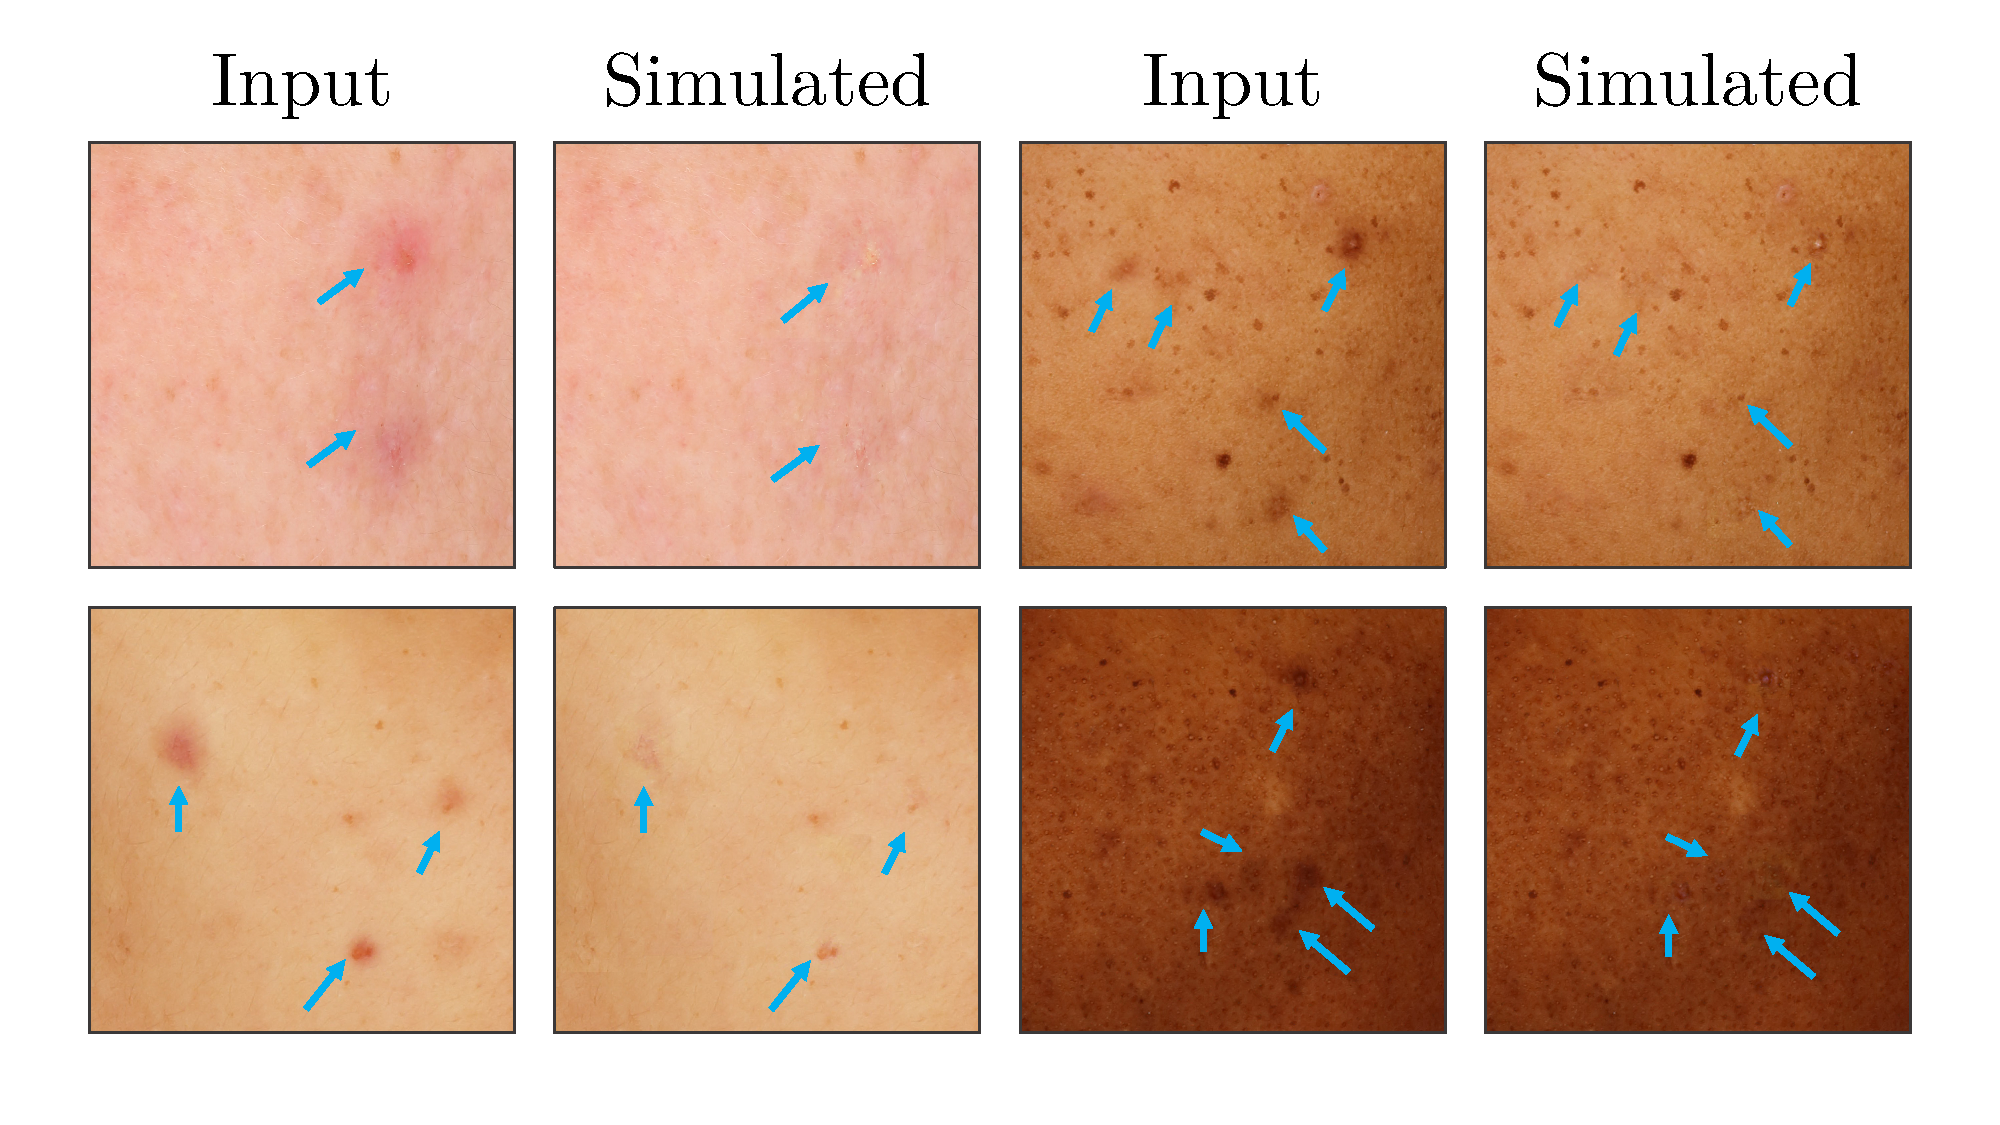
\includegraphics[width=\columnwidth]{Chapter5/img_comp4.pdf}
    \caption{Simulation under various skin tones}
    \label{fig:sim1}
\end{figure}

\section{Reality}
\begin{figure}[t!]
    \centering
    % \begin{subfigure}
    %     \centering
        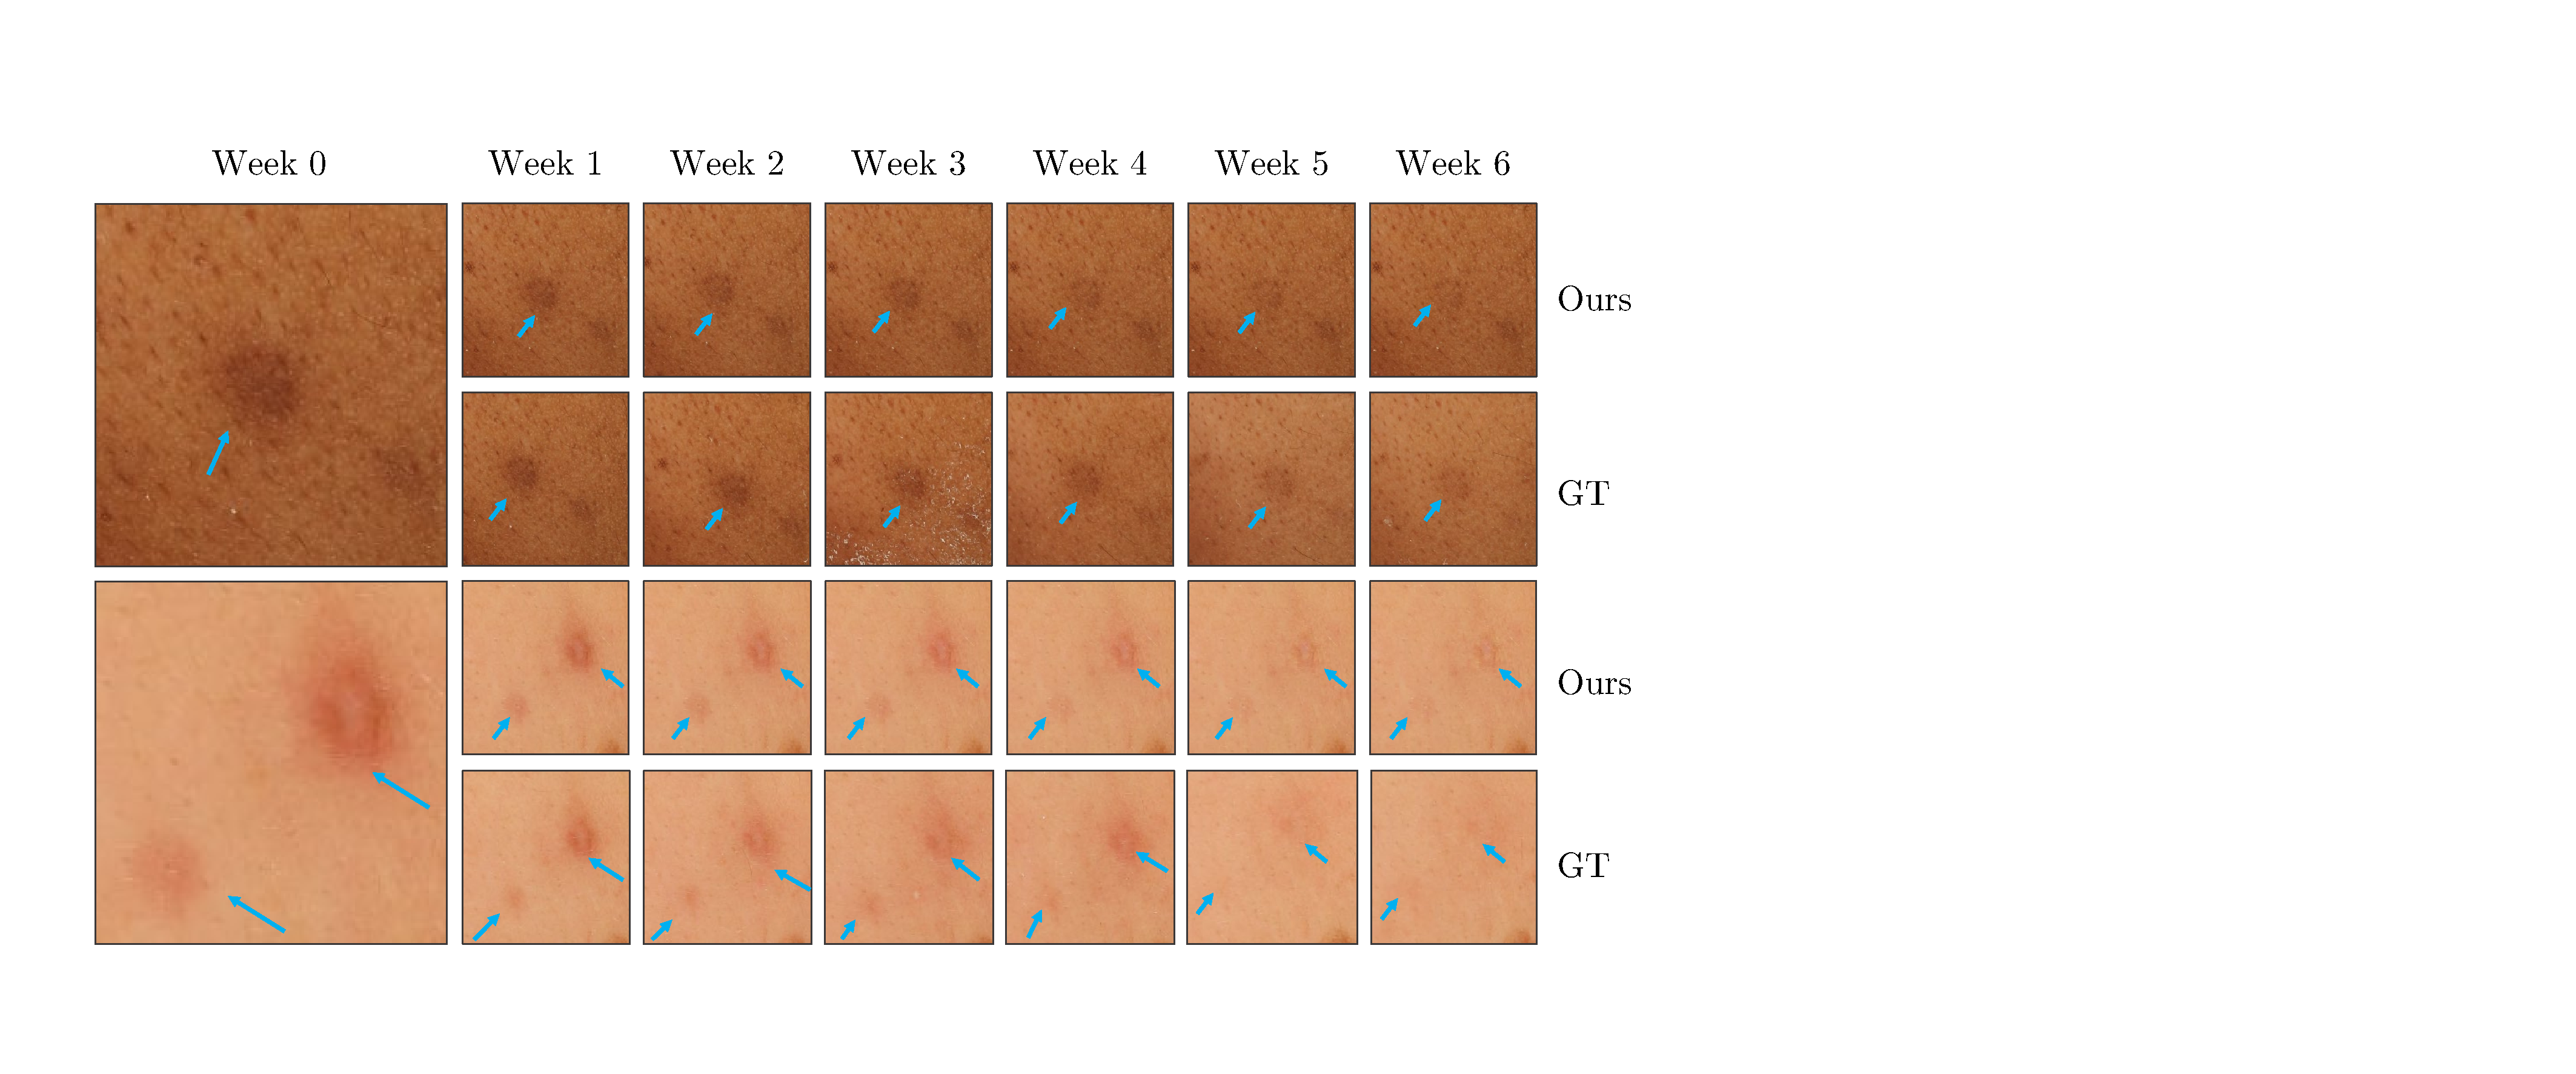
\includegraphics[width=\columnwidth]{Chapter5/forward3.pdf}
        \caption{Simulation of blemish fading process}
    % \end{subfigure}
    % \vspace{2em}

    \caption{The application of the proposed method to the simulation of the fading process of skin blemish is shown. Blue Arrows are manually added to highlight blemishes of interest (acne or pigmentation). In the simulation, images of \textit{Week 0} are input and the parameters of the obtained model are adjusted to simulate the change of the blemishes in the following weeks. Note that the proposed method applies to different skin tones and various types of blemishes.}
    \label{fig:forward}
\end{figure}
Exploration of reality evaluates the proposed algorithm's ability to simulate complex changes in real human skin conditions. Some skin blemish samples with long-term evolution patterns from the dataset are selected and simulated using the proposed algorithm. Figure \ref{fig:forward} shows one example, revealing the gradual fading of pigmentations over 7 weeks. The proposed algorithm successfully simulates the natural fading trajectory of the pigmentations, showing a natural change in color.

For the PS method, the inpainting tool of the software is utilized, selecting and removing blemishes on the original image under the Content-Aware mode. The modified image is then combined with the original image through Alpha blending. For the SD method, the inpainting mode is used and the text prompt is set as \texttt{skin patch, human face skin, high definition, best quality}. Each test is performed with 50 iterations of sampling using the \texttt{DPM++SDE Karras} sampler, with the random seed fixed to 42. The denoising ratio is adjusted to increase the difference between the generated image and the original.

Fréchet Inception Distance (FID) scores for the simulated images and the ground-truth images are calculated to quantitatively measure the quality of algorithms for skin blemish editing. The results are displayed in Table \ref{tbl:fid} and the visual comparison is shown in Figure \ref{fig:baseline}.
\begin{figure}[t!]
    \centering
    \begin{subfigure}{.9\textwidth}
        \centering
        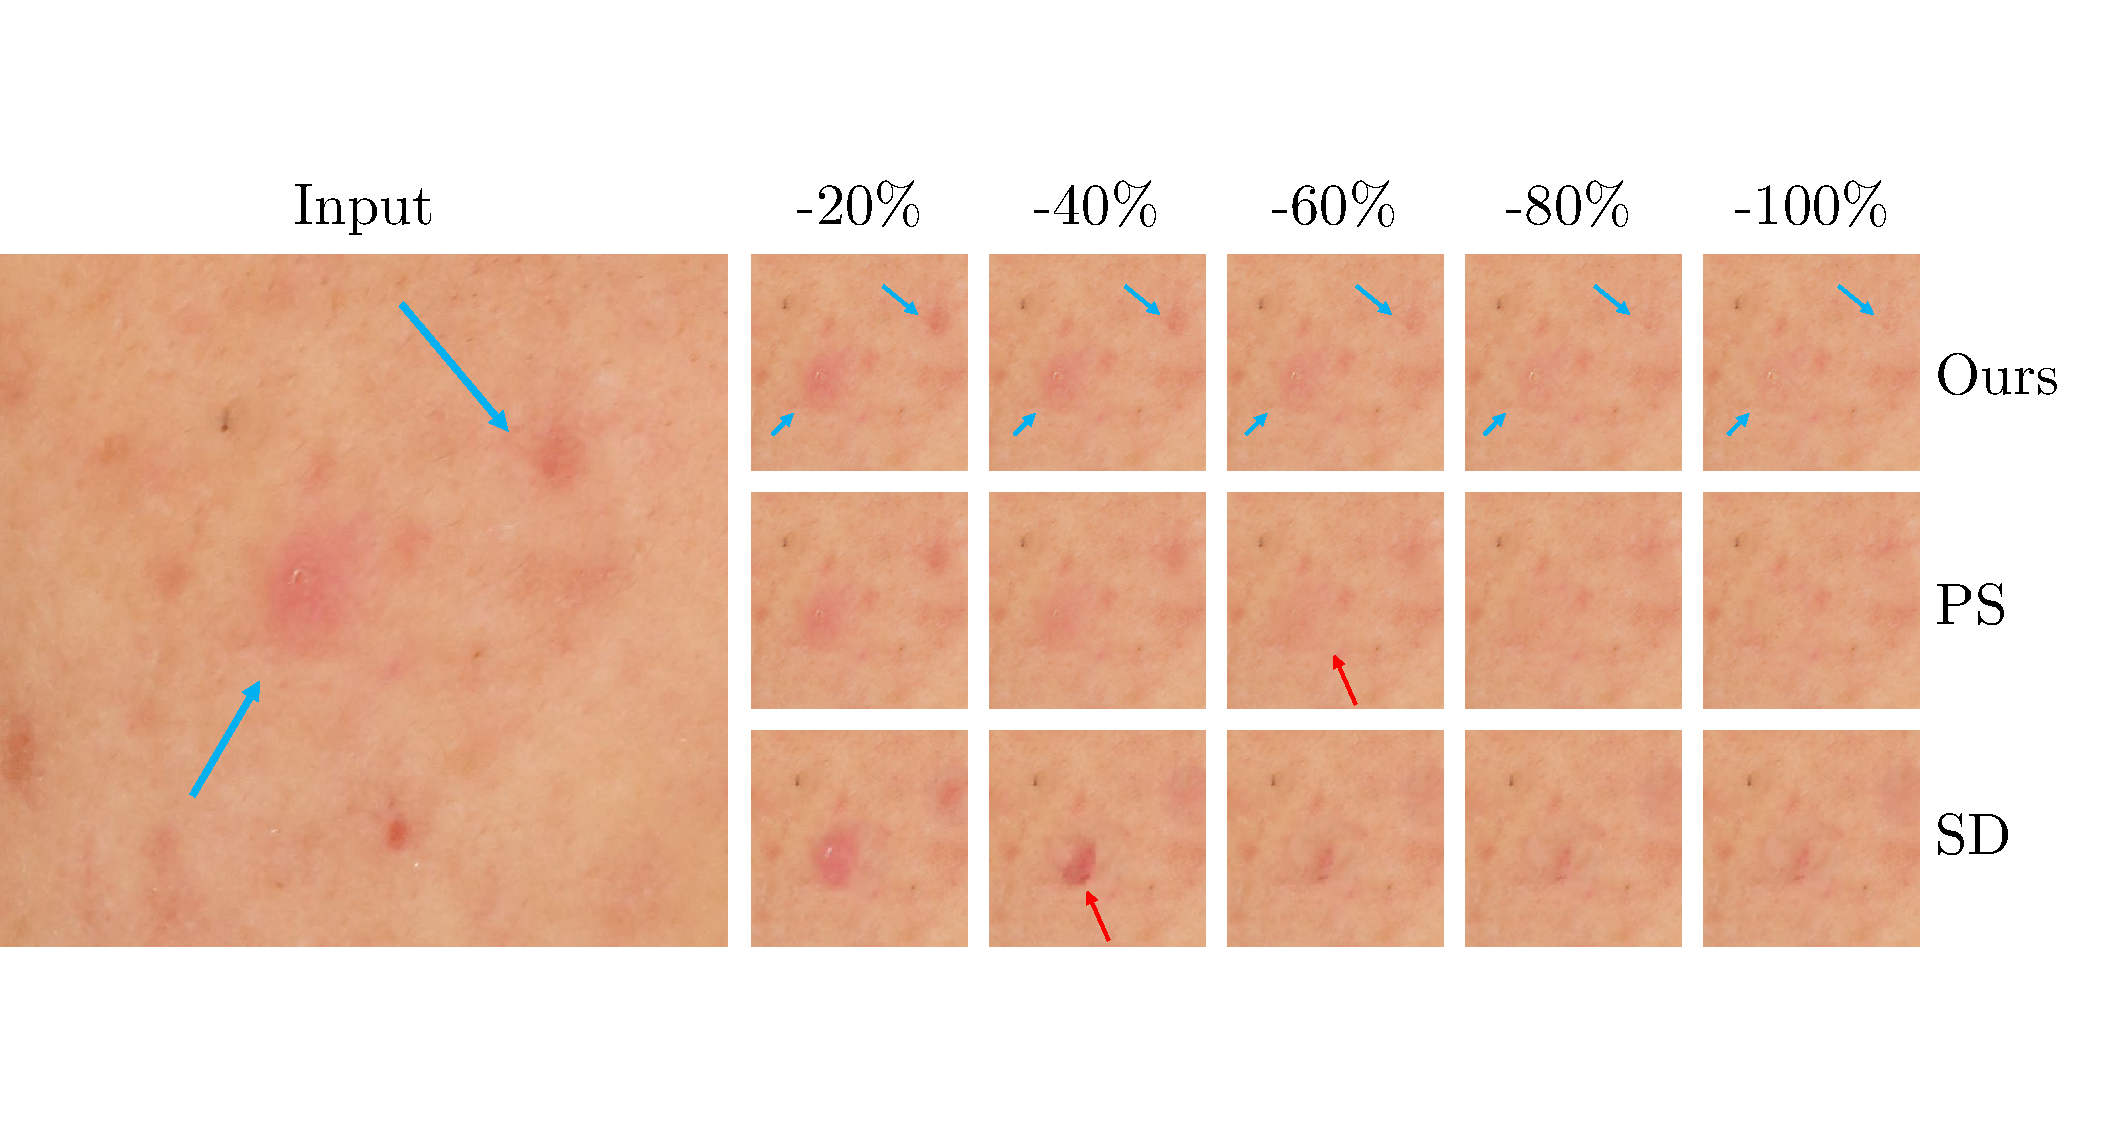
\includegraphics[width=\linewidth]{Chapter5/baseline11.pdf}
    \end{subfigure}
    \hfill
    \begin{subfigure}{.9\textwidth}
        \centering
        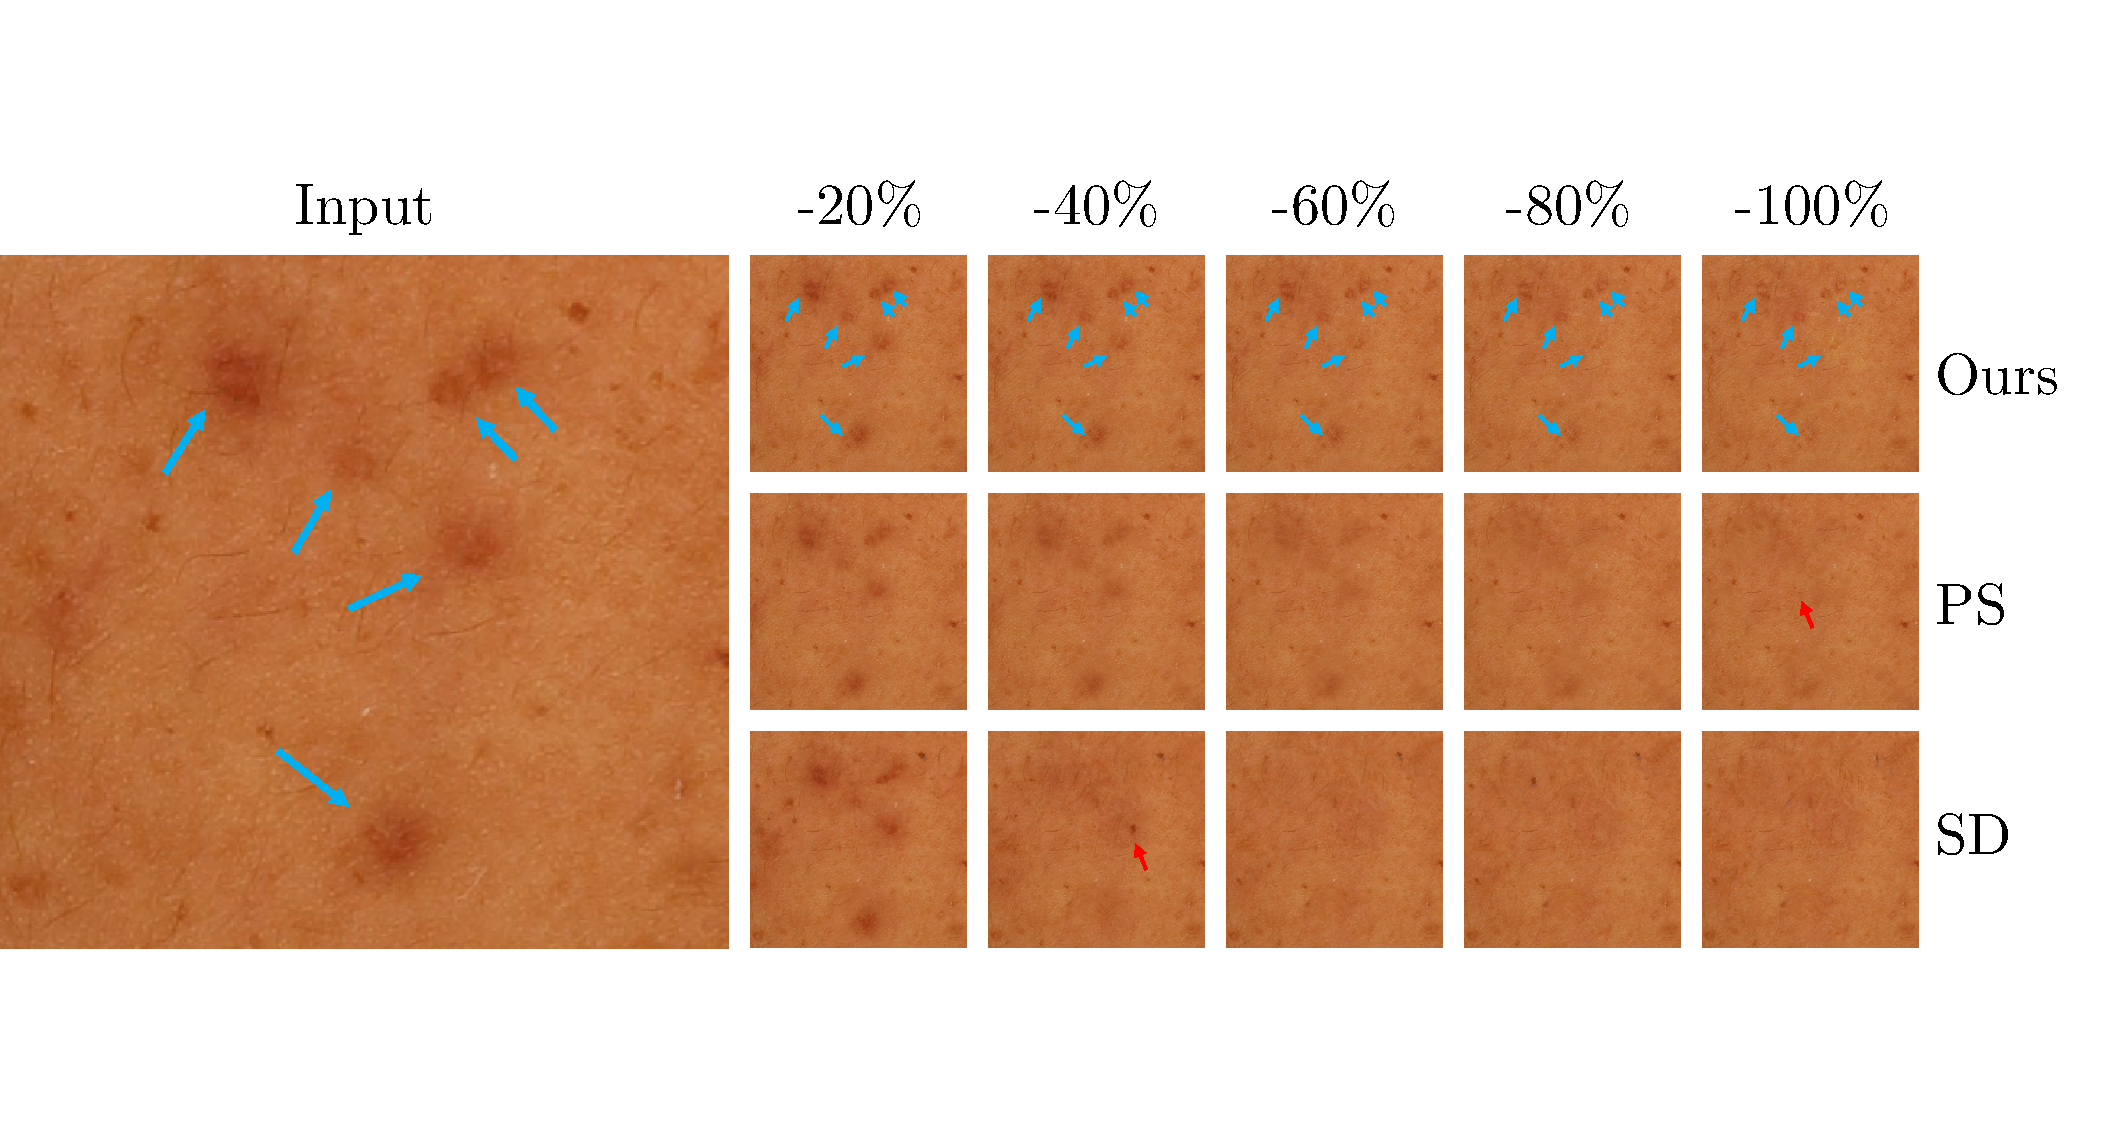
\includegraphics[width=\linewidth]{Chapter5/baseline12.pdf}
    \end{subfigure}
    \caption{Comparison with baseline methods. The results of several blemish removal or modification methods are compared, including the proposed method in question (marked as Ours), Adobe Photoshop\cite{adobephotoshop} inpainting (marked as PS), and Stable Diffusion\cite{rombach2021highresolution} inpainting (marked as SD). Arrows are manually added to highlight areas of interest. Note the red arrows where the PS produces over-smoothed skin patches and the SD produces visible artifacts.}
    \label{fig:baseline}
\end{figure}

\begin{table}[t!]
    \caption{FID scores of different blemish fading rates. Lower scores are better.}
    \resizebox{\columnwidth}{!}{%
        \begin{tabular}{cccccc}
            \hline
            \multirow{2}{*}{Methods} & \multicolumn{5}{c}{Fading Rate}                                                                         \\ \cline{2-6}
                                     & 100\%                           & 80\%            & 60\%            & 40\%            & 20\%            \\ \hline\hline
            SD                       & 144.89                          & 133.53          & 134.16          & 160.10          & 159.54          \\
            PS                       & 117.98                          & 120.37          & 125.15          & 129.26          & \textbf{129.96} \\
            \textbf{Proposed}            & \textbf{115.30}                 & \textbf{118.12} & \textbf{122.64} & \textbf{127.09} & 131.60          \\ \hline
        \end{tabular}%
    }
    \label{tbl:fid}
\end{table}

For the FID scores, the proposed method achieved the lowest scores in the vast majority of cases, except for the 20\% fading rate. In particular, the proposed method has less variation in FID scores compared to other baselines at different fading rates, which suggests that the proposed model is able to achieve robust, realistic skin blemish simulations.

Visual comparison more intuitively demonstrates the superiority of the proposed algorithm. The PS method, although straightforward, led to a loss of skin detail through simple interpolation, resulting in blurry patches. Conversely, the SD method generated some contextually coherent skin details while removing the blemishes, but its quality was limited. Specifically, at higher denoising ratios, the SD method produced noticeable artifacts, and the modified areas differed in color from the surrounding skin.

The proposed method not only closely aligns with the natural degradation process of real skin but also ensures that the modified pigmentations match the underlying skin seamlessly. Unlike other techniques, this approach does not create artifacts or blurriness. It maintains skin details, including subtle textures such as hair and pores, leading to a natural appearance. This underlines the effectiveness of the proposed method in preserving the intricacy of skin texture while accomplishing realistic modifications.

\begin{figure}[t!]
    \centering
    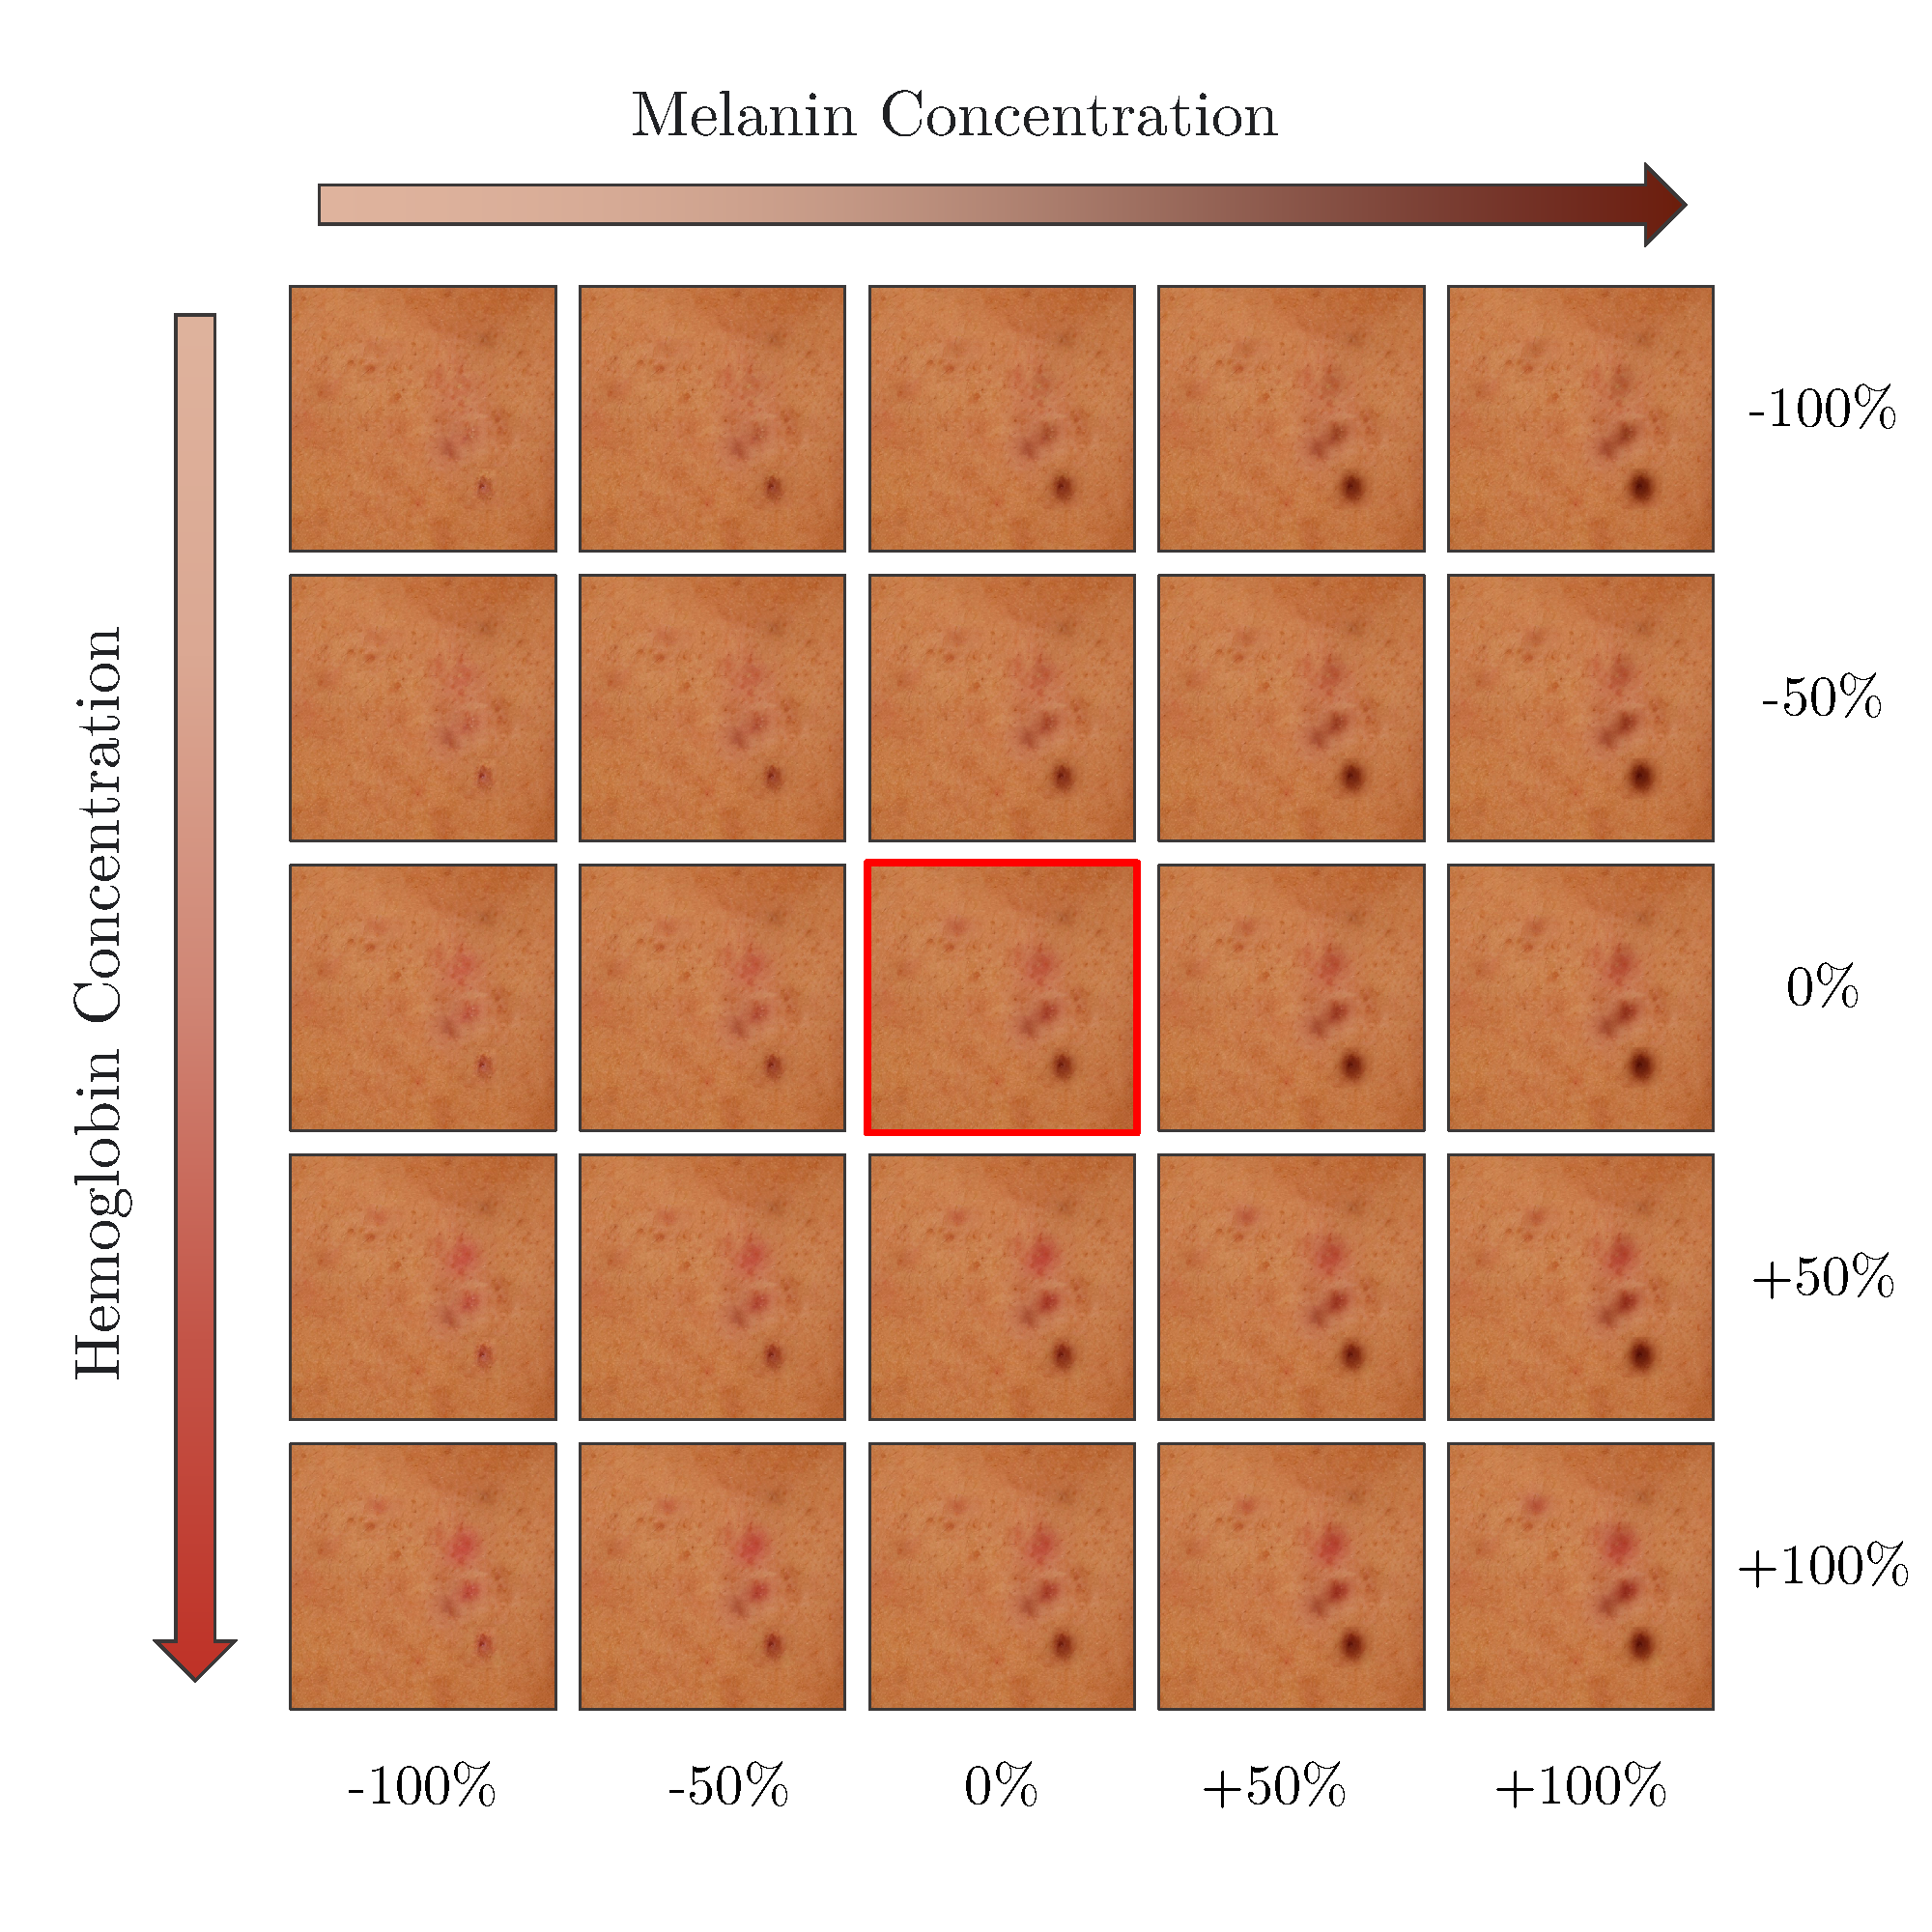
\includegraphics[width=0.96\columnwidth]{Chapter5/grid.pdf}
    \caption{Matrix of different chromophore concentrations setting. The original image is marked by a red box. The proposed model fully decouples the major chromophores of human skin, enabling highly controllable pigmentation editing.}
    \label{fig:matrix}
\end{figure}

\section{Controllability}
Controllability is key to user interaction with the proposed algorithm. A significant advantage of the proposed model is its high controllability, where users can freely adjust the parameters of the pigmentation to precisely control its appearance.
A changing matrix is plotted by adjusting the concentration control parameters of melanin and heamoglobin, as shown in Figure \ref{fig:matrix}. The proposed method successfully decouples the concentrations of these two chromophores, allowing users to independently control their apparent features, thus flexibly simulating the change of blemishes under different conditions.

\section{Perception Study}
\begin{figure}[t!]
    \centering
    \begin{subfigure}{.9\textwidth}
        \centering
        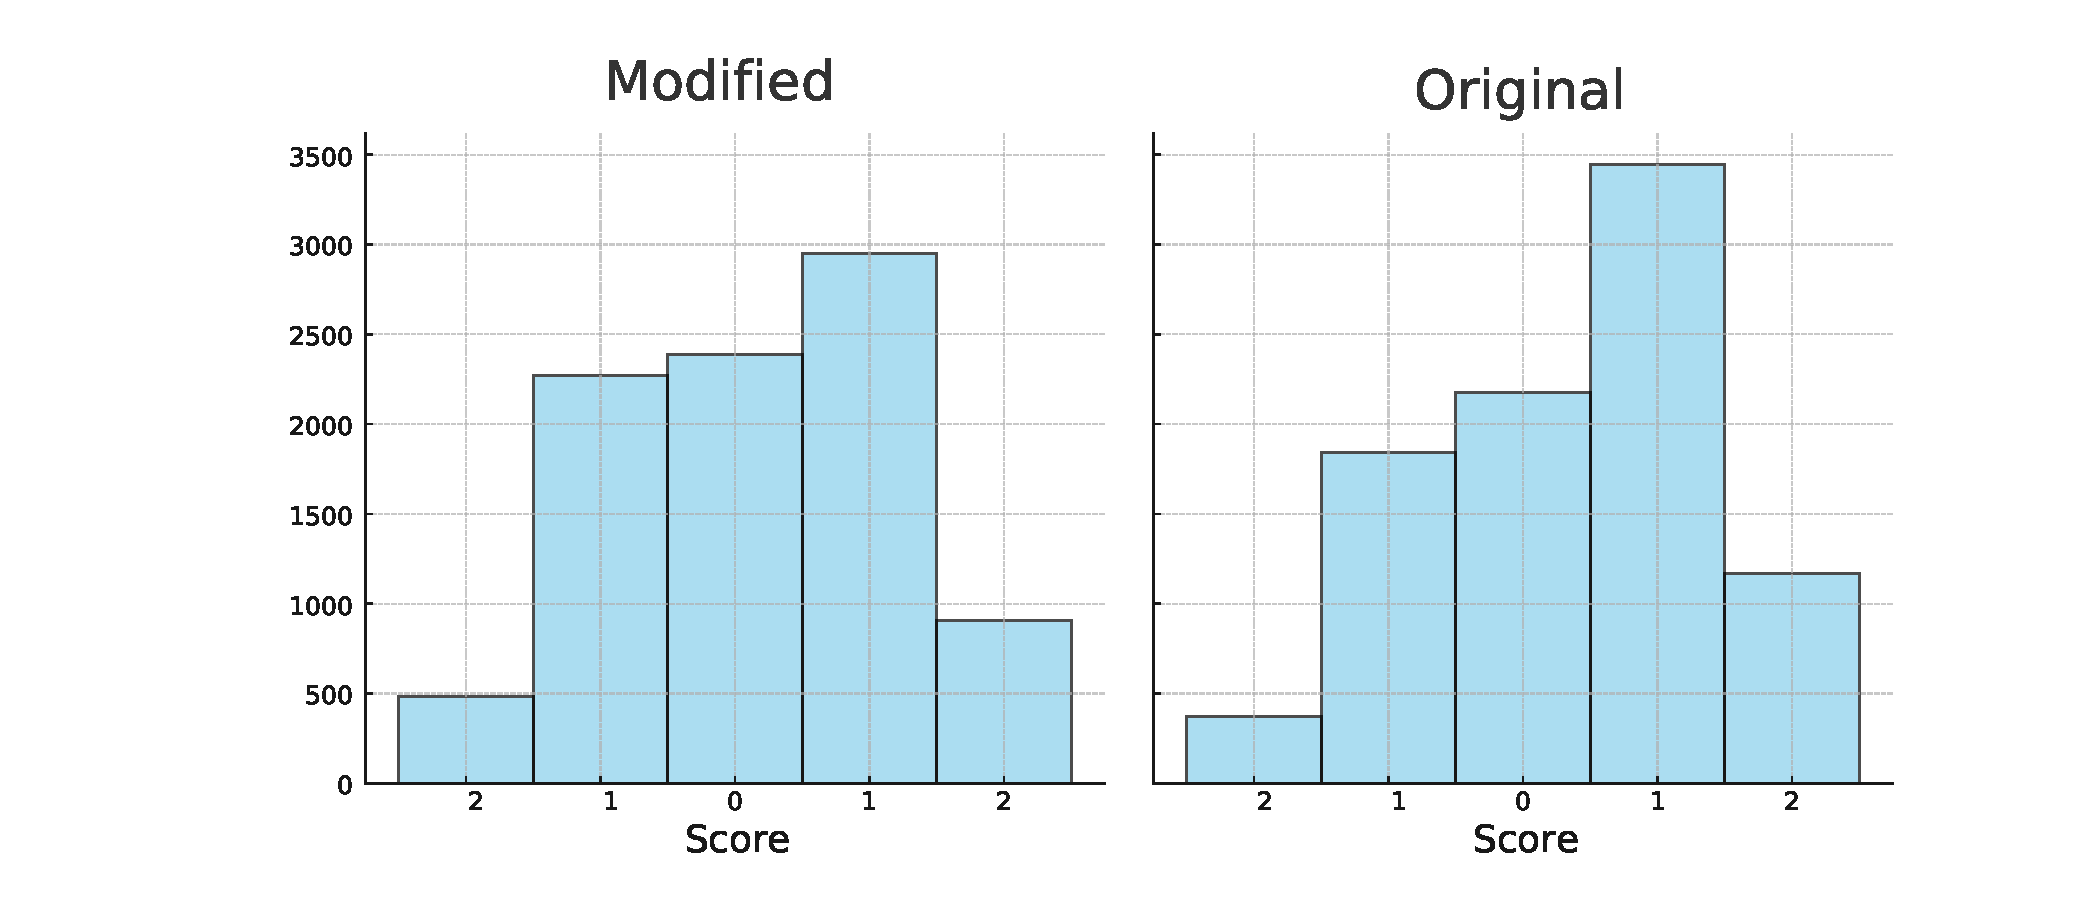
\includegraphics[width=0.95\columnwidth]{Chapter5/score.pdf}
        \caption{Scoring frequencies of survey responses}
        \label{fig:survey_hist}
    \end{subfigure}\hfill
    \begin{subfigure}{.9\textwidth}
        \centering
        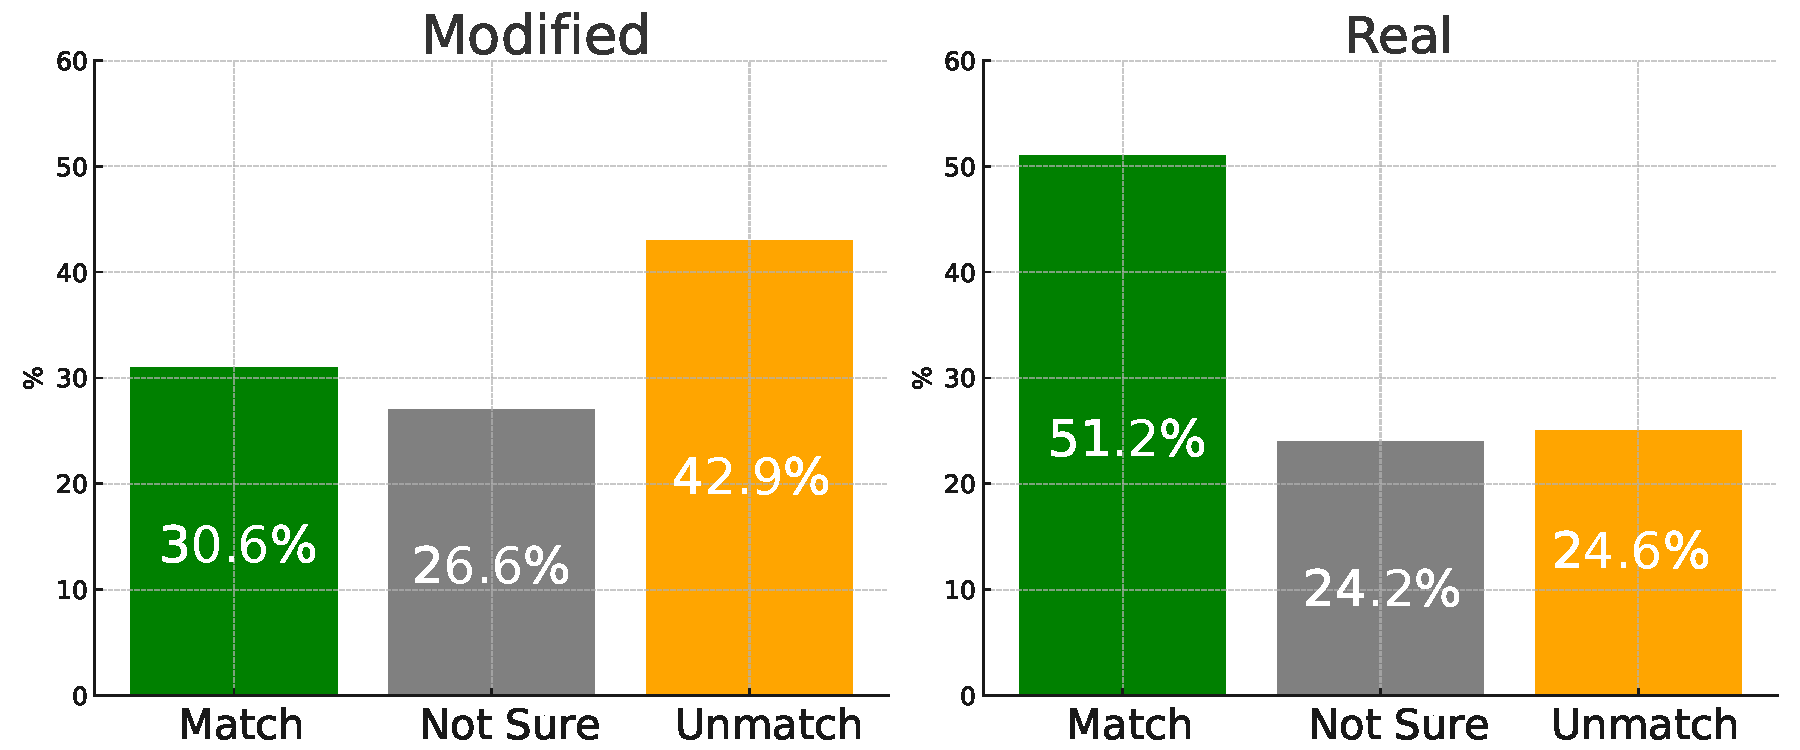
\includegraphics[width=0.95\columnwidth]{Chapter5/bar_charts_modified.pdf}
        \caption{Bar chart of survey results}
        \label{fig:bar_charts}
    \end{subfigure}
    \caption{Panellists scored images from -2 to +2 to assess their confidence in considering the image as modified or not, with higher scores indicating that the user considered the image to be unmodified. Scoring frequencies are displayed in Figure \ref{fig:survey_hist}. The results of the survey are shown in Figure \ref{fig:bar_charts}. For the modified images, more people perceived them as unmodified or not sure. This suggests that the modifications are consistent with human perception and intuition.}
\end{figure}
The objective of this study is to evaluate if the pigmentation simulation is natural and believable. As shown in Figure \ref{fig:bar_charts}, the altered images had a lower average score (0.16956 vs 0.35511), with only 30.6\% correctly identifying the altered image vs 23.6\% judging the real images as altered, and 26.6\% not sure if it is or is not altered. This indicates that the effect of the proposed algorithm is superior, to the point where laypeople cannot readily discern traces of algorithmic alteration.

%=== END OF CHAPTER FIVE ===
\end{spacing}
\newpage

%=== CHAPTER SIX (6) ===
%=== Conclusion and Recommendations ===

\chapter{Conclusion \& Future Work}
\begin{spacing}{1.5}
\setlength{\parskip}{0.3in}

% A novel method for simulating skin spot changes is proposed, utilizing a physics-based model coupled with expertise in dermatology, to successfully achieve the modeling of facial skin blemishes. Based on this, an efficient system for precise simulation of blemish changes over an extended period is developed, facilitating highly controllable, natural, and authentic adjustments to the appearance of blemishes. Experiments demonstrate that this algorithm is broadly applicable to various skin tones and types of pigmentations. In comparison to learning-based image manipulation algorithms, this method does not require learning pigmentation patterns from large data sets, yet can achieve results that are comparable in quality.

% This method also has limitations. For instance, it requires users to manually select the blemish area rather than being able to predict their locations automatically. Moreover, the user study highlighted that while a significant percentage of the altered images were perceived as realistic, there remains a portion of images where the alterations were detectable. This underscores the need for continuous improvement in the simulation's subtlety and realism, particularly when dealing with high variability in human perception. Additionally, the parameter settings have only been tested and validated on a self-collected dataset, and whether the proposed algorithm can be applied to images captured in the wild with more complex lighting situations requires further verification.

% In conclusion, this research carves new possibilities in the cosmetic industry. With future improvements, this method has the potential to drive innovation and customization in skin care products, meeting the ever-growing demands of consumers. This work is hopeful to provide valuable insights and inspiration for future exploration in the cross-disciplinary field of computer vision and skin science.
\section{Conclusion}
In conclusion, the novel method presented in this research for simulating skin blemish changes marks a significant advancement in the realm of dermatological technology. By utilizing a physics-based model enriched with dermatological expertise, this approach successfully models facial skin blemishes, offering a highly controllable, natural, and authentic simulation of blemish changes over time. This system, demonstrating broad applicability across various skin tones and blemishes, stands out for its ability to achieve quality results without relying on extensive learning from large datasets, a common limitation in many learning-based image manipulation algorithms.

However, the method is not without its challenges. The requirement for manual selection of blemish areas points to a need for automation in future iterations, potentially through the integration of advanced detection algorithms. Additionally, the user study results suggest a necessity for refining the simulation's subtlety to enhance its realism further, particularly in the face of diverse human perceptions. The parameter settings, while effective within the scope of a controlled dataset, warrant additional testing in more variable, real-world scenarios to ensure broader applicability and reliability.

\section{Future Work}
Looking ahead, this research opens up new pathways in the skincare industry, particularly in the development of skincare products. The potential for this method to foster innovation and customization is significant, aligning well with the evolving demands of consumers seeking personalized skincare solutions. Moreover, the insights gained from this research could act as a catalyst for future interdisciplinary explorations, bridging the gap between computer vision and skin science. The development of more sophisticated, user-friendly, and versatile tools for skin blemish simulation and analysis could bring benefits for both consumer experience and dermatological research. As this field continues to evolve, the integration of machine vision, and image processing with dermatological knowledge will likely unveil new horizons in skincare and treatment, potentially transforming both daily skincare routines and professional dermatological practices.

%=== END OF CHAPTER SIX ===
\end{spacing}
    
\newpage

%==== ENDING PART ===

\renewcommand\bibname{References}
\bibliographystyle{unsrt}
\begin{spacing}{1.5}
\bibliography{Ref/References}
\end{spacing}
\newpage

%=== APPENDIX ===

\begin{appendices}
\label{cha:appendices}

\chapter{Simulation on Various Skin Tones}
\markboth{Appendix A}{} % For appendix first (affects header)
% sadsadsadsadsadsadsadsadsa
\begin{spacing}{1.5}
\vspace{-2em}
The proposed model's performance on different skin tones is displayed here. In each set, the left image is the input, and the right image is the output. Arrows indicate the pigmentation or acne of interest, selected by the panellists. These chosen skin blemishes are completely removed by the proposed model. Zoom in for a better view.
% \vspace{-0.5em}
\begin{figure}[h]
    \begin{subfigure}{.5\textwidth}
        \centering
        \includegraphics[width=.9\linewidth]{Appendix/img/1.pdf}
        \caption{Dark}
      \end{subfigure}%
      \begin{subfigure}{.5\textwidth}
        \centering
        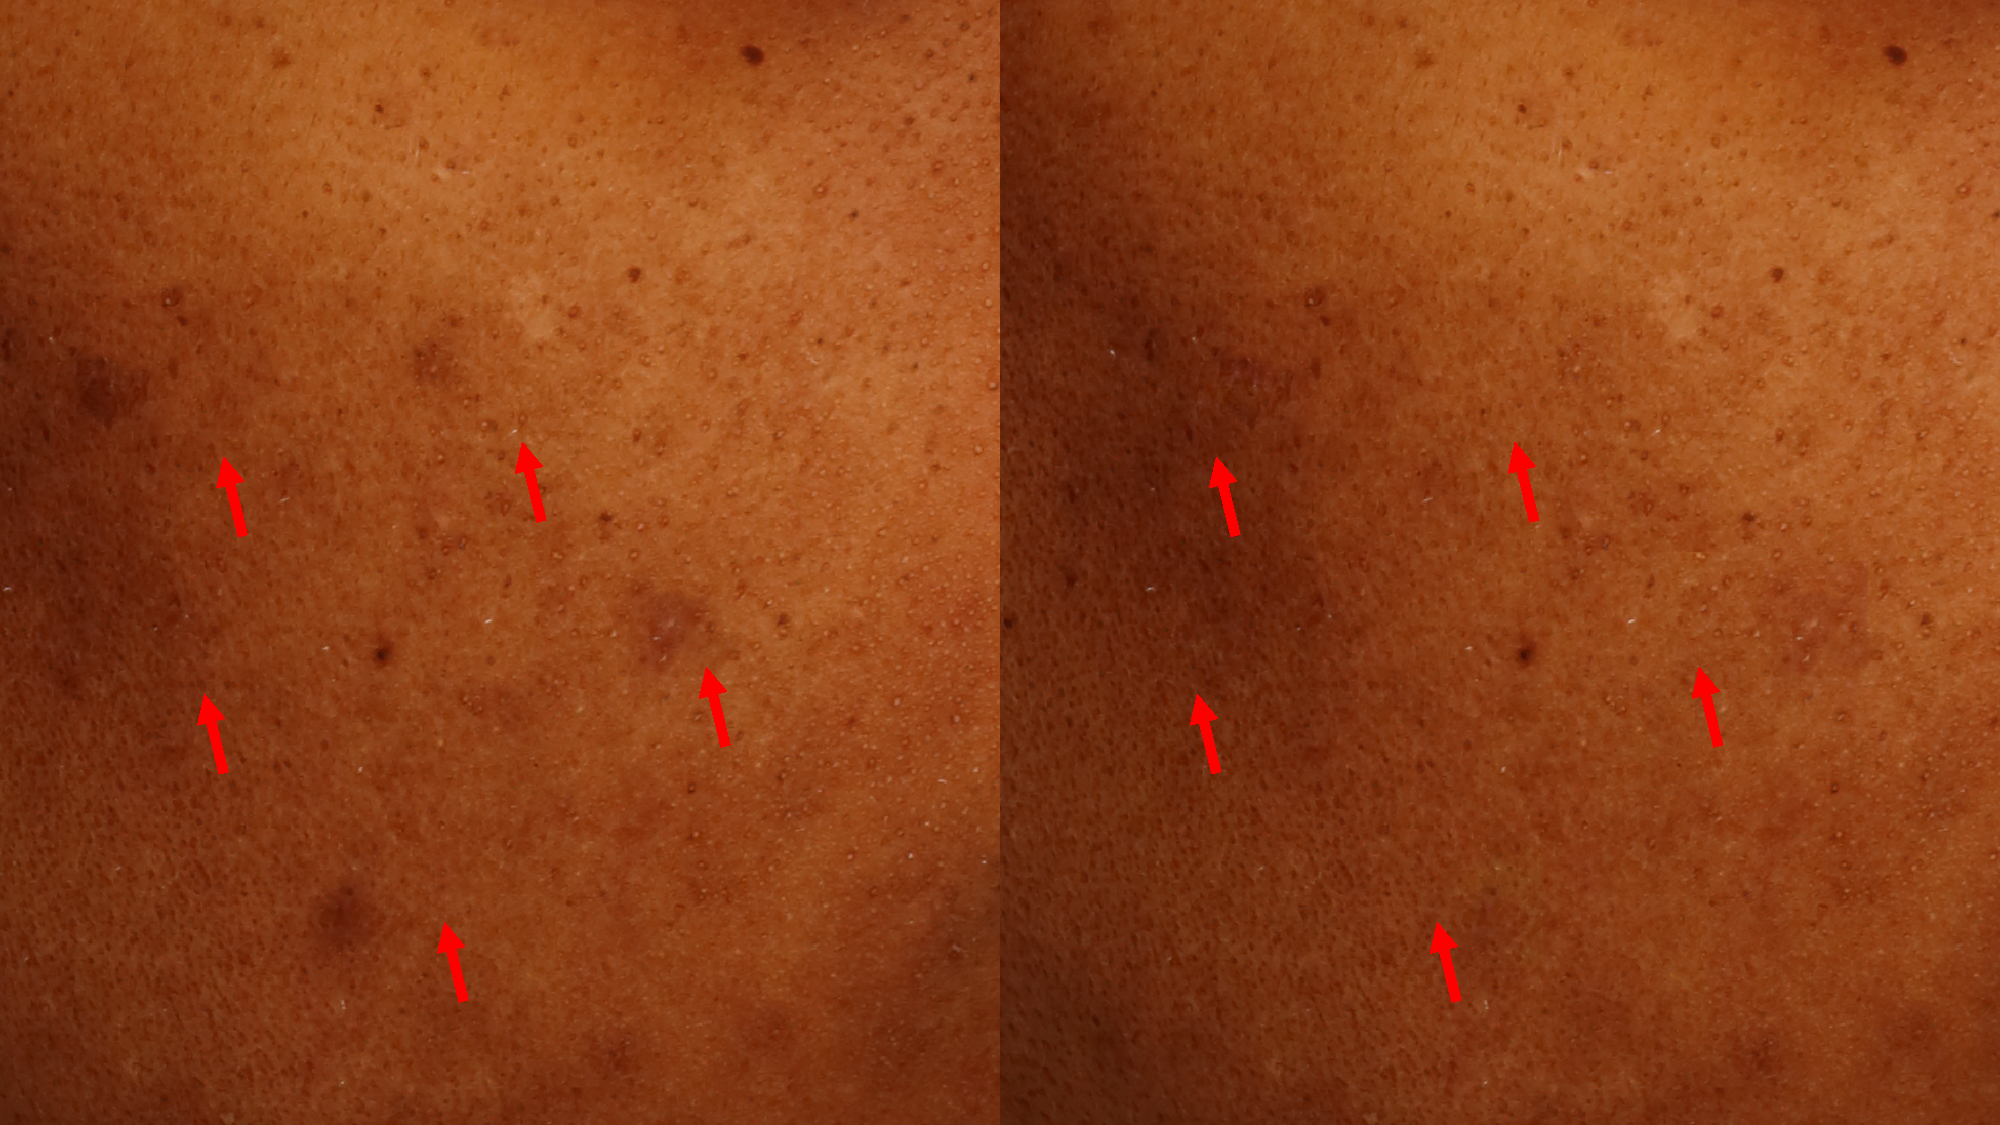
\includegraphics[width=.9\linewidth]{Appendix/img/2.pdf}
        \caption{Dark}
      \end{subfigure}
    \begin{subfigure}{.5\textwidth}
        \centering
        \includegraphics[width=.9\linewidth]{Appendix/img/3.pdf}
        \caption{Dark}
      \end{subfigure}%
      \begin{subfigure}{.5\textwidth}
        \centering
        \includegraphics[width=.9\linewidth]{Appendix/img/4.pdf}
        \caption{Dark}
      \end{subfigure}
    \begin{subfigure}{.5\textwidth}
        \centering
        \includegraphics[width=.9\linewidth]{Appendix/img/5.pdf}
        \caption{Brown}
      \end{subfigure}%
      \begin{subfigure}{.5\textwidth}
        \centering
        \includegraphics[width=.9\linewidth]{Appendix/img/6.pdf}
        \caption{Brown}
      \end{subfigure}
\end{figure}
\begin{figure}[p]\ContinuedFloat
    \begin{subfigure}{.5\textwidth}
        \centering
        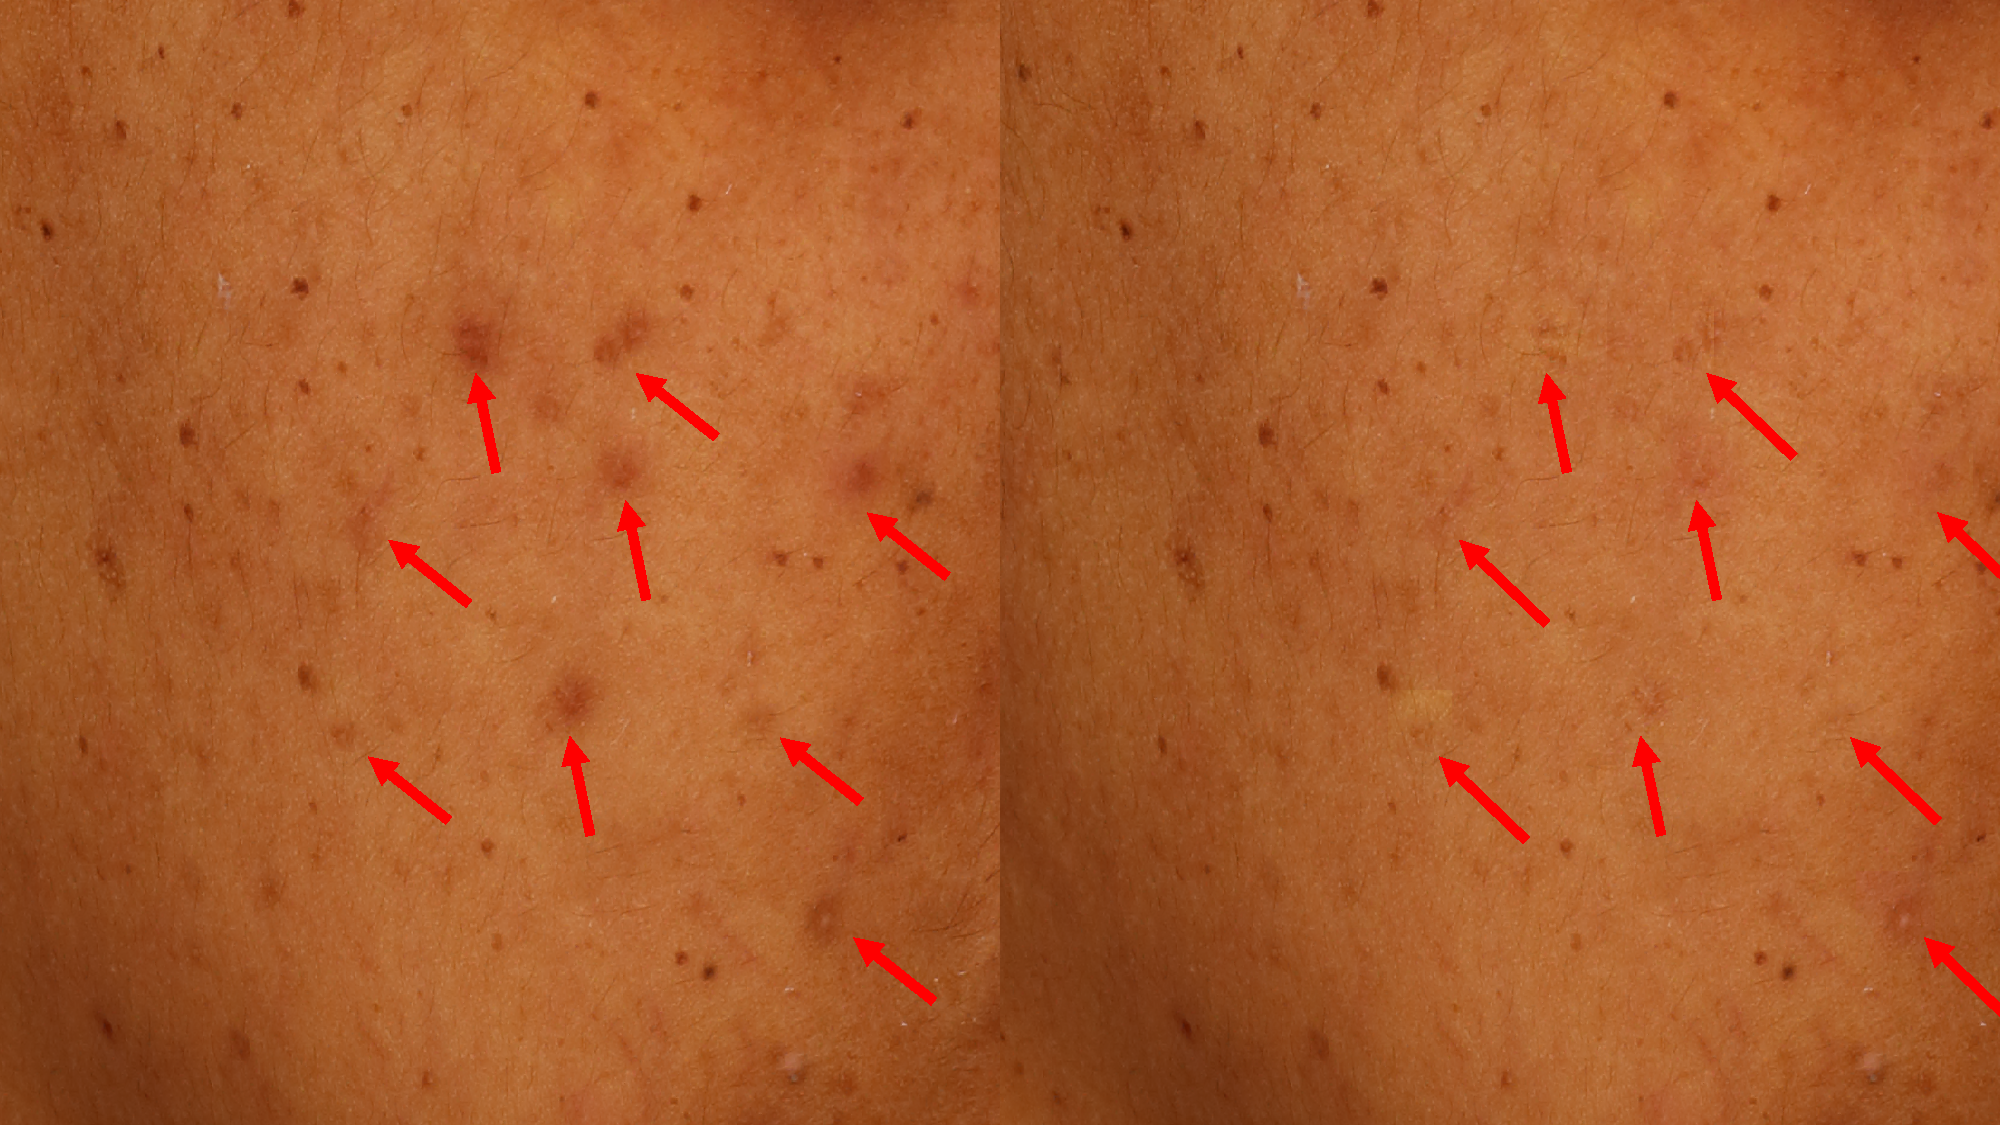
\includegraphics[width=.9\linewidth]{Appendix/img/7.pdf}
        \caption{Brown}
      \end{subfigure}%
      \begin{subfigure}{.5\textwidth}
        \centering
        \includegraphics[width=.9\linewidth]{Appendix/img/8.pdf}
        \caption{Brown}
      \end{subfigure}
    \begin{subfigure}{.5\textwidth}
        \centering
        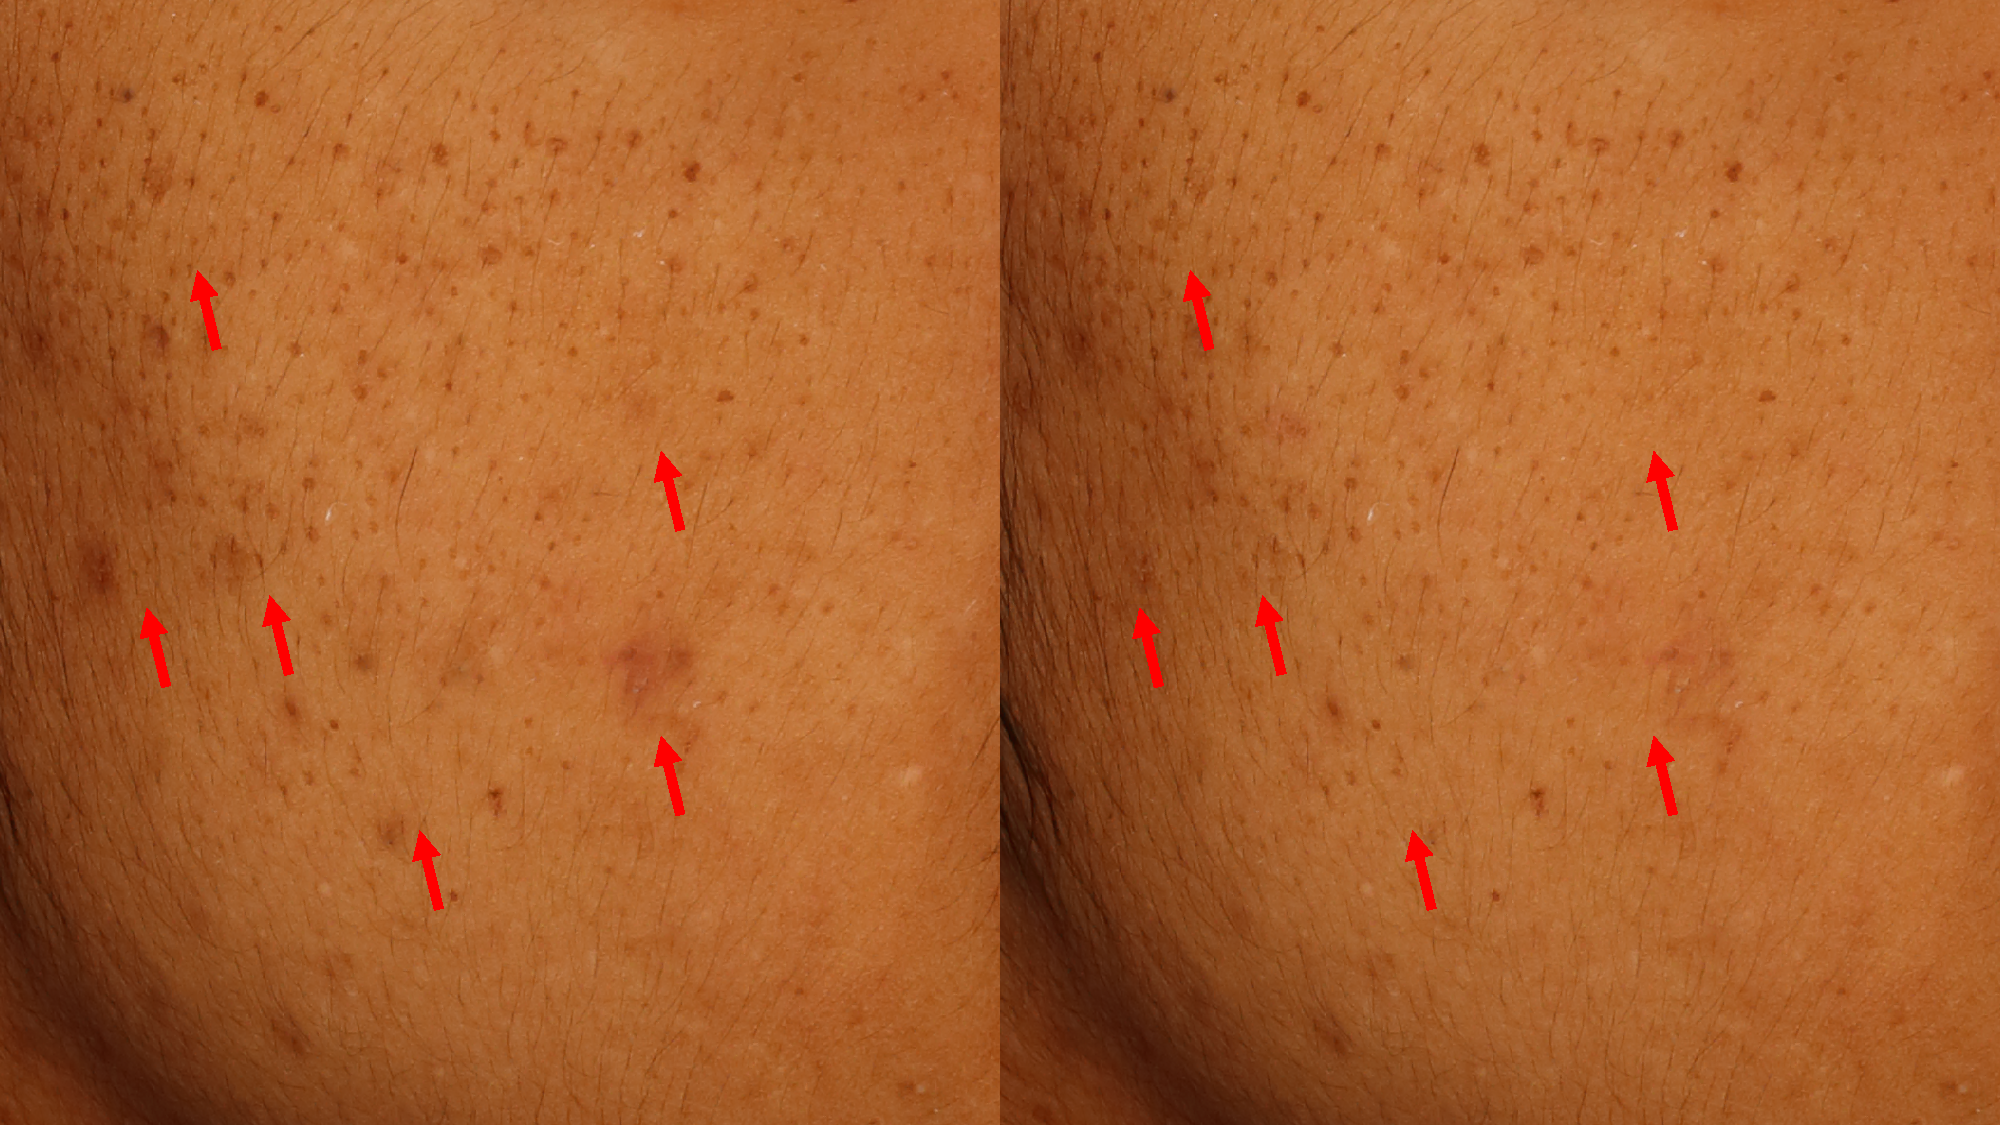
\includegraphics[width=.9\linewidth]{Appendix/img/9.pdf}
        \caption{Brown}
      \end{subfigure}%
      \begin{subfigure}{.5\textwidth}
        \centering
        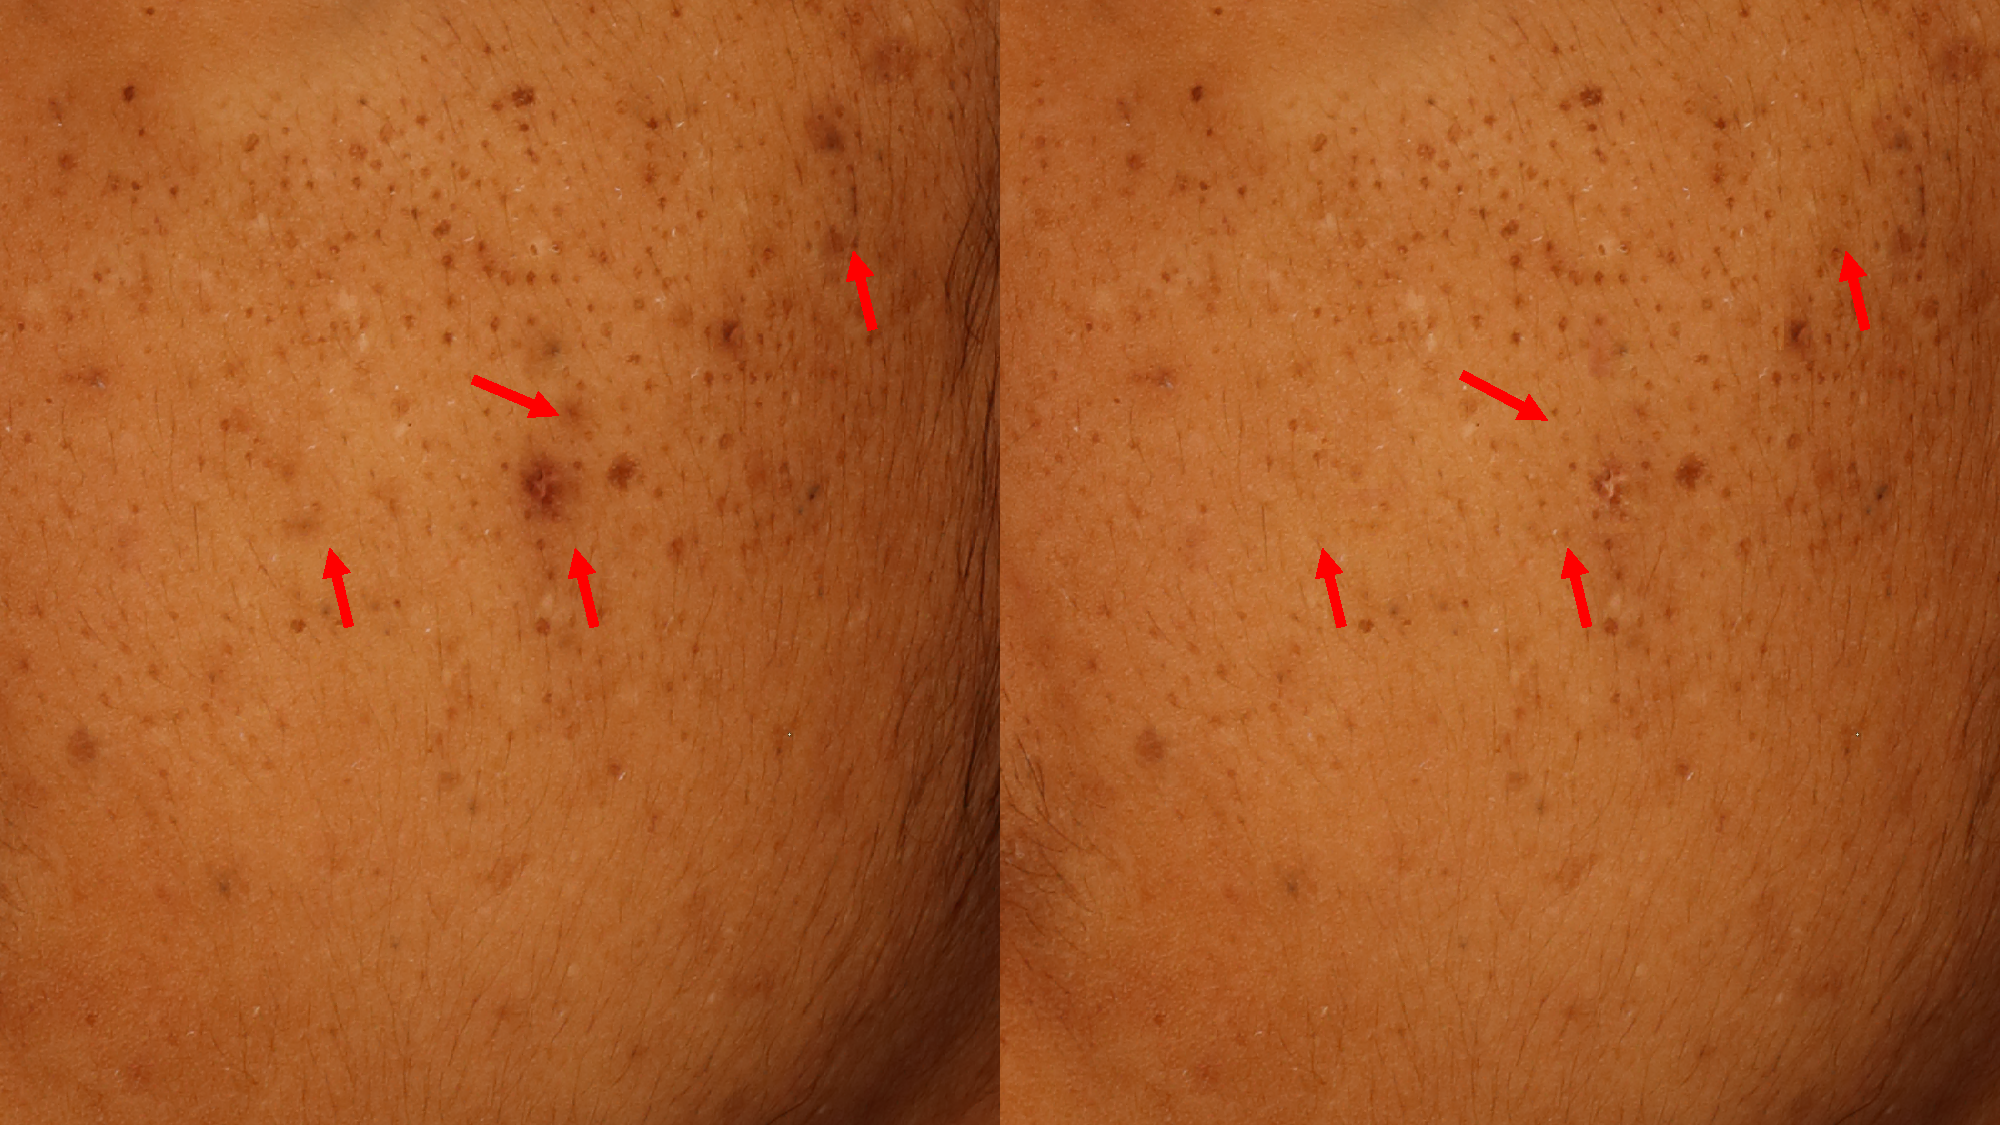
\includegraphics[width=.9\linewidth]{Appendix/img/10.pdf}
        \caption{Brown}
      \end{subfigure}
    \begin{subfigure}{.5\textwidth}
        \centering
        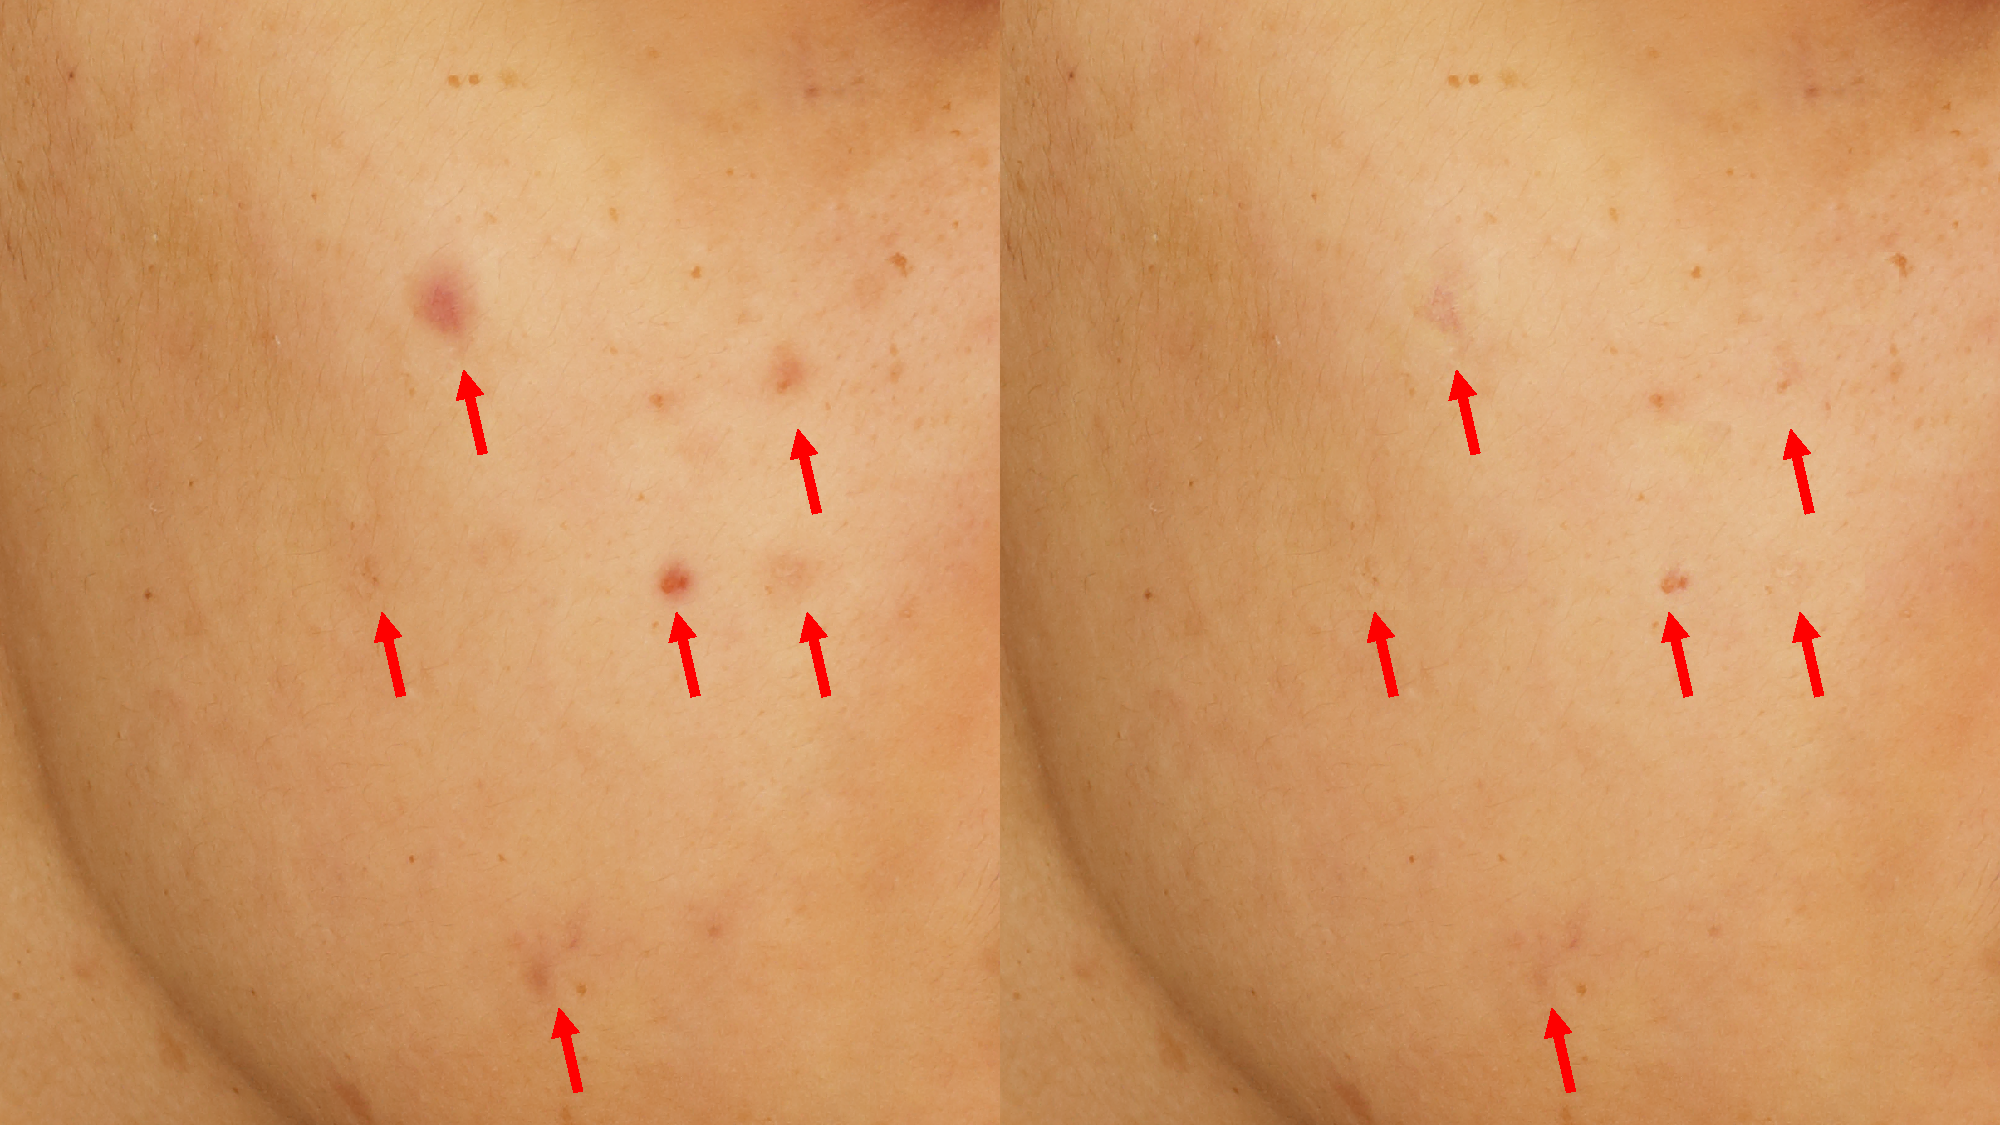
\includegraphics[width=.9\linewidth]{Appendix/img/11.pdf}
        \caption{Intermediate}
      \end{subfigure}%
      \begin{subfigure}{.5\textwidth}
        \centering
        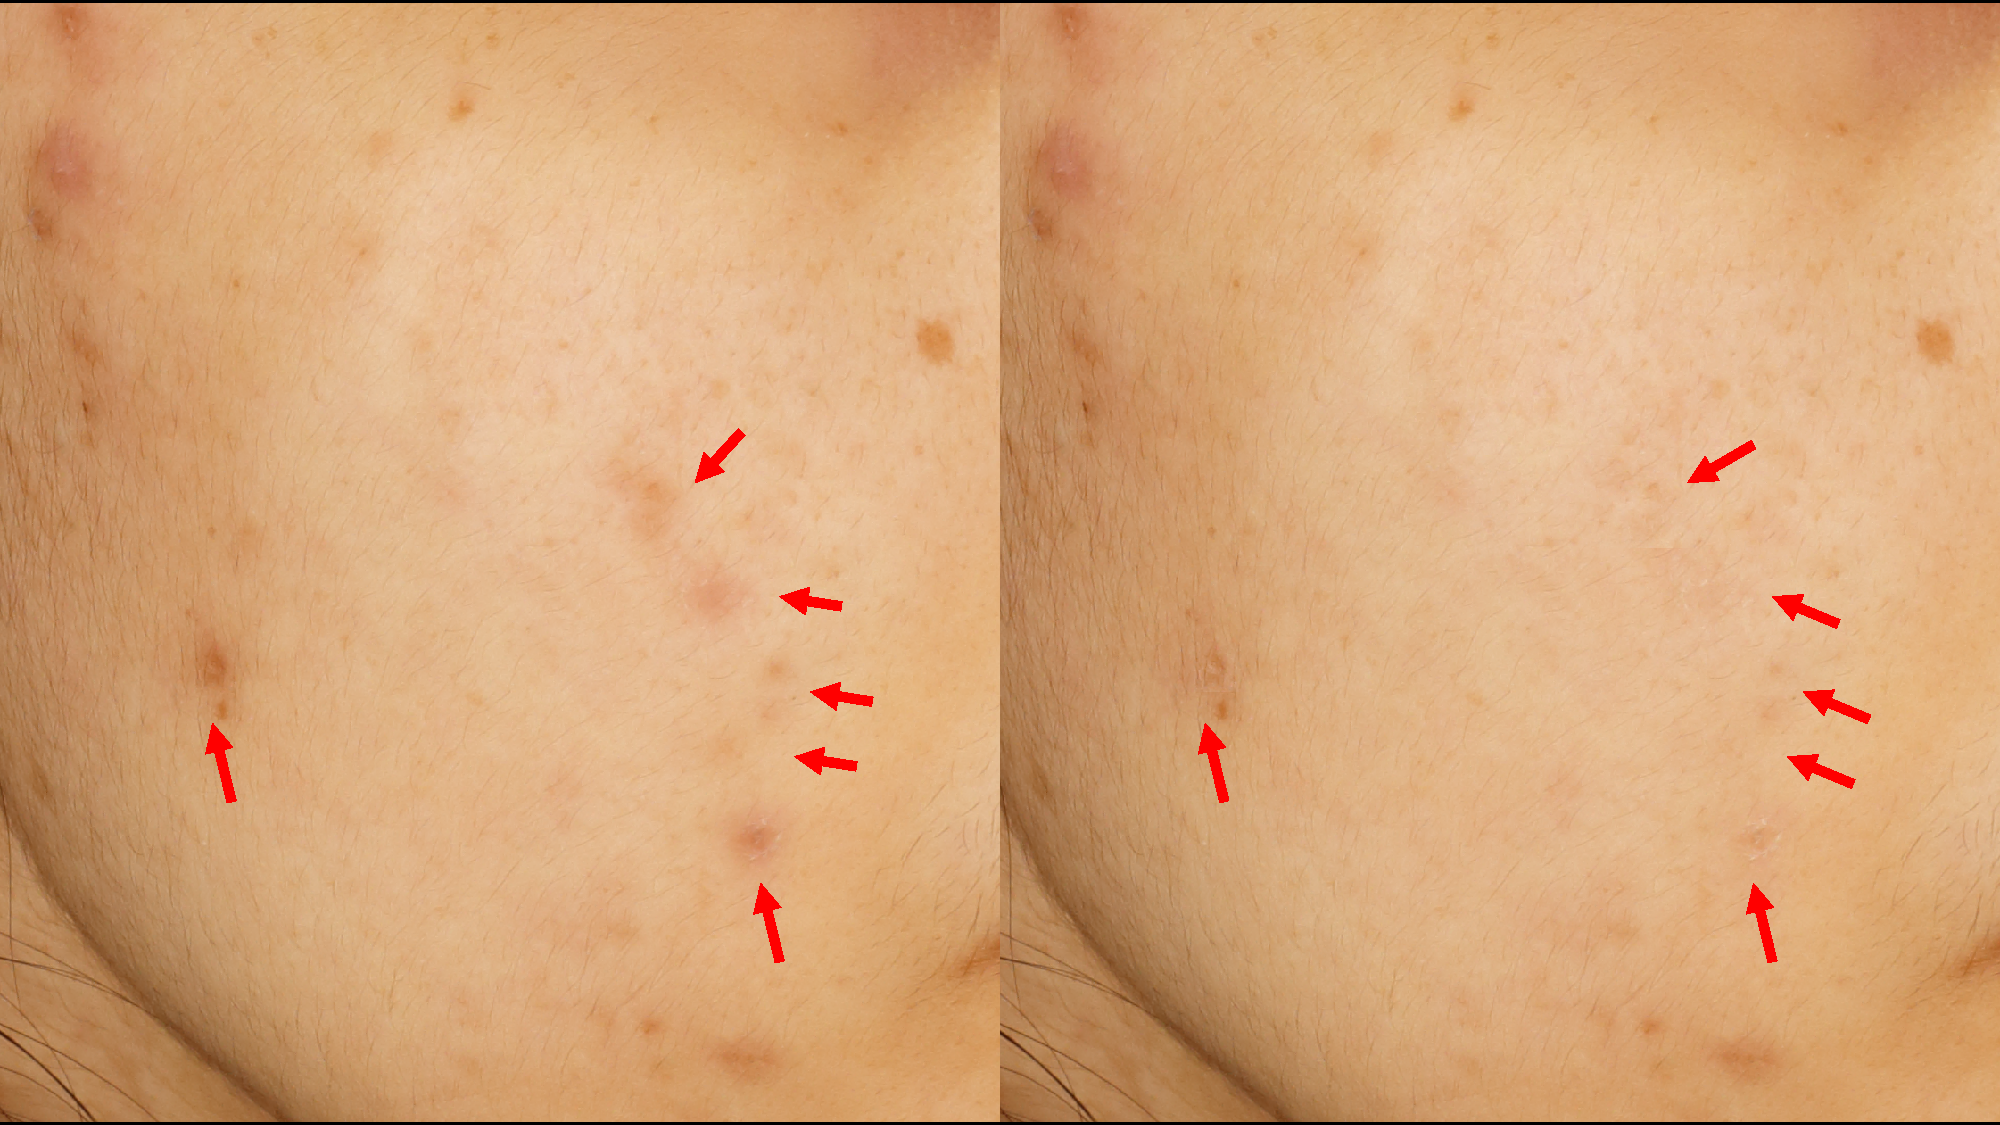
\includegraphics[width=.9\linewidth]{Appendix/img/12.pdf}
        \caption{Intermediate}
      \end{subfigure}
    \begin{subfigure}{.5\textwidth}
        \centering
        \includegraphics[width=.9\linewidth]{Appendix/img/13.pdf}
        \caption{Light}
      \end{subfigure}%
      \begin{subfigure}{.5\textwidth}
        \centering
        \includegraphics[width=.9\linewidth]{Appendix/img/14.pdf}
        \caption{Light}
      \end{subfigure}
    \begin{subfigure}{.5\textwidth}
        \centering
        \includegraphics[width=.9\linewidth]{Appendix/img/15.pdf}
        \caption{Tan}
      \end{subfigure}%
      \begin{subfigure}{.5\textwidth}
        \centering
        \includegraphics[width=.9\linewidth]{Appendix/img/16.pdf}
        \caption{Tan}
      \end{subfigure}
\end{figure}
\end{spacing}

% \chapter{Sample Code}
% \markboth{Appendix B}{} % For appendix second, etc.. 

% below shows how to insert highlighted source code from the source file.

% \inputminted[
% tabsize=4, % change this to set the spacing of tab
% breaklines, % automatically wrap the code
% fontsize=\scriptsize % Can be \footnotesize, \small, \normalsize etc
% ]{python}{Appendix/sample.py}

\end{appendices}
%==== END OF ALL ===
\end{document}
